% VLDB template version of 2020-08-03 enhances the ACM template, version 1.7.0:
% https://www.acm.org/publications/proceedings-template
% The ACM Latex guide provides further information about the ACM template

\documentclass[sigconf, nonacm]{acmart}

%% The following content must be adapted for the final version
% paper-specific
\newcommand\vldbdoi{XX.XX/XXX.XX}
\newcommand\vldbpages{XXX-XXX}
% issue-specific
\newcommand\vldbvolume{19}
\newcommand\vldbissue{1}
\newcommand\vldbyear{2026}
% should be fine as it is
\newcommand\vldbauthors{\authors}
\newcommand\vldbtitle{\shorttitle} 
% leave empty if no availability url should be set
\newcommand\vldbavailabilityurl{https://github.com/balajinix/map-reflect}
% whether page numbers should be shown or not, use 'plain' for review versions, 'empty' for camera ready
\newcommand\vldbpagestyle{plain} 

\usepackage{xcolor}
\usepackage{graphicx}
\usepackage{tabularx}
\usepackage{enumitem}
\usepackage{booktabs}
\usepackage{balance}
\newcolumntype{R}{>{\raggedleft\arraybackslash}X}
\graphicspath{{./}{charts/}}

% Relax line breaking to reduce overfull hbox warnings
\tolerance=1000
\emergencystretch=3em
\hfuzz=1.5pt
\widowpenalty=10000
\clubpenalty=10000

\newcommand{\as}[1]{\textcolor{blue}{#1}}
\newcommand{\bg}[1]{\textcolor{brown}{#1}}
\newcommand{\cg}[1]{\textcolor{red}{#1}}
\newcommand{\deleted}[1]{\textcolor{red}{#1}}
\newcommand{\added}[1]{\textcolor{blue}{#1}}

\begin{document}
\title{Map-Reflect: Uncertainty-Guided Reflection for Schema Mapping}

%%
%% The "author" command and its associated commands are used to define the authors and their affiliations.
\author{Balaji Ganesan$^{*}$}
%\orcid{0000-0001-5109-3700}
\affiliation{%
  \institution{IBM Software}
  \country{India}
}
\email{bganesa1@in.ibm.com}

\author{Avirup Saha$^{*}$}
\affiliation{%
  \institution{IBM Software}
  \country{India}
}
\email{avirup.saha2@ibm.com}

\author{Gunjan Siddharth$^{\dagger}$}
%\orcid{0000-0002-1825-0097}
\affiliation{%
  \institution{Vellore Institute of Technology}
  \country{India}
}
\email{gunjan.siddharth2022@vitstudent.ac.in}

\author{Ravindran Jagannathan}
\affiliation{%
  \institution{IBM Software}
  \country{USA}
}
\email{ravi.jagannathan@ibm.com}

\author{Amit Paradkar}
\affiliation{%
  \institution{IBM Software}
  \country{USA}
}
\email{paradkar@us.ibm.com}

\author{Pratibha Moogi} 
\affiliation{%
  \institution{IBM Software}
  \country{India}
}
\email{pratibha.moogi@ibm.com}


%%
%% The abstract is a short summary of the work to be presented in the
%% article.
\begin{abstract}
Schema mapping is the task of aligning database tables, API endpoints, and GraphQL types together with their fields across heterogeneous schemas. It is a prerequisite for data federation, function calling, and agentic tool composition. LLM-based approaches increasingly use reflection to improve mapping quality, but a key open question is \emph{when} reflection helps and when it hurts. We show empirically that most reflection triggers degrade accuracy: structural signals and heuristic error detectors fire on already-correct predictions and cause the model to over-correct. Only uncertainty-guided reflection consistently avoids this degradation, making it the safe default across diverse benchmarks. We introduce Map-Reflect, an \emph{gated reflection} framework that operationalises this finding. Map-Reflect is schema-agnostic and works with REST APIs, GraphQL, and relational databases. It supports runtime target discovery without elaborate offline pre-processing and runs with open-source models. We also introduce ITOpsGraph and ITOpsGraph-MB, the first benchmarks for enterprise API schema mapping with heterogeneous paradigms (GraphQL and proto buffer) and human-annotated many-to-many ground truth, filling a gap that existing relational benchmarks cannot address.
\end{abstract}

\renewcommand{\shortauthors}{Ganesan and Saha, et al.}

\maketitle
{\renewcommand{\thefootnote}{\fnsymbol{footnote}}\footnotetext[1]{Equal contribution.}\footnotetext[2]{Work done at IBM.}}

%%% do not modify the following VLDB block %%
%%% VLDB block start %%%
\pagestyle{\vldbpagestyle}
\begingroup\small\noindent\raggedright\textbf{PVLDB Reference Format:}\\
\vldbauthors. \vldbtitle. PVLDB, \vldbvolume(\vldbissue): \vldbpages, \vldbyear.\\
\href{https://doi.org/\vldbdoi}{doi:\vldbdoi}
\endgroup
\begingroup
\renewcommand\thefootnote{}\footnote{\noindent
This work is licensed under the Creative Commons BY-NC-ND 4.0 International License. Visit \url{https://creativecommons.org/licenses/by-nc-nd/4.0/} to view a copy of this license. For any use beyond those covered by this license, obtain permission by emailing \href{mailto:info@vldb.org}{info@vldb.org}. Copyright is held by the owner/author(s). Publication rights licensed to the VLDB Endowment. \\
\raggedright Proceedings of the VLDB Endowment, Vol. \vldbvolume, No. \vldbissue\ %
ISSN 2150-8097. \\
\href{https://doi.org/\vldbdoi}{doi:\vldbdoi} \\
}\addtocounter{footnote}{-1}\endgroup
%%% VLDB block end %%%

%%% do not modify the following VLDB block %%
%%% VLDB block start %%%
\ifdefempty{\vldbavailabilityurl}{}{
\vspace{.3cm}
\begingroup\small\noindent\raggedright\textbf{PVLDB Artifact Availability:}\\
The source code, data, and/or other artifacts have been made available at \url{\vldbavailabilityurl}.
\endgroup
}
%%% VLDB block end %%%

\section{Introduction}
\label{sec:intro}
Organizations rely on diverse API ecosystems and databases that must be integrated for effective data access. Schema mapping~\cite{matchmaker,liu2024magneto,sheetrit2024rematch,buss2025scalableschemamappingusing,lenzerini2002data,halevy2006data,doan2012principles}, is the task of identifying equivalent entity types across different schemas, and is critical for building unified data access layers that allow querying across heterogeneous sources without knowledge of the underlying schema differences. This matters for AI agents and tool-calling scenarios~\cite{wang2024llmagent}, where LLMs must select and invoke APIs across multiple services.

\begin{figure}[!t]
    \centering
    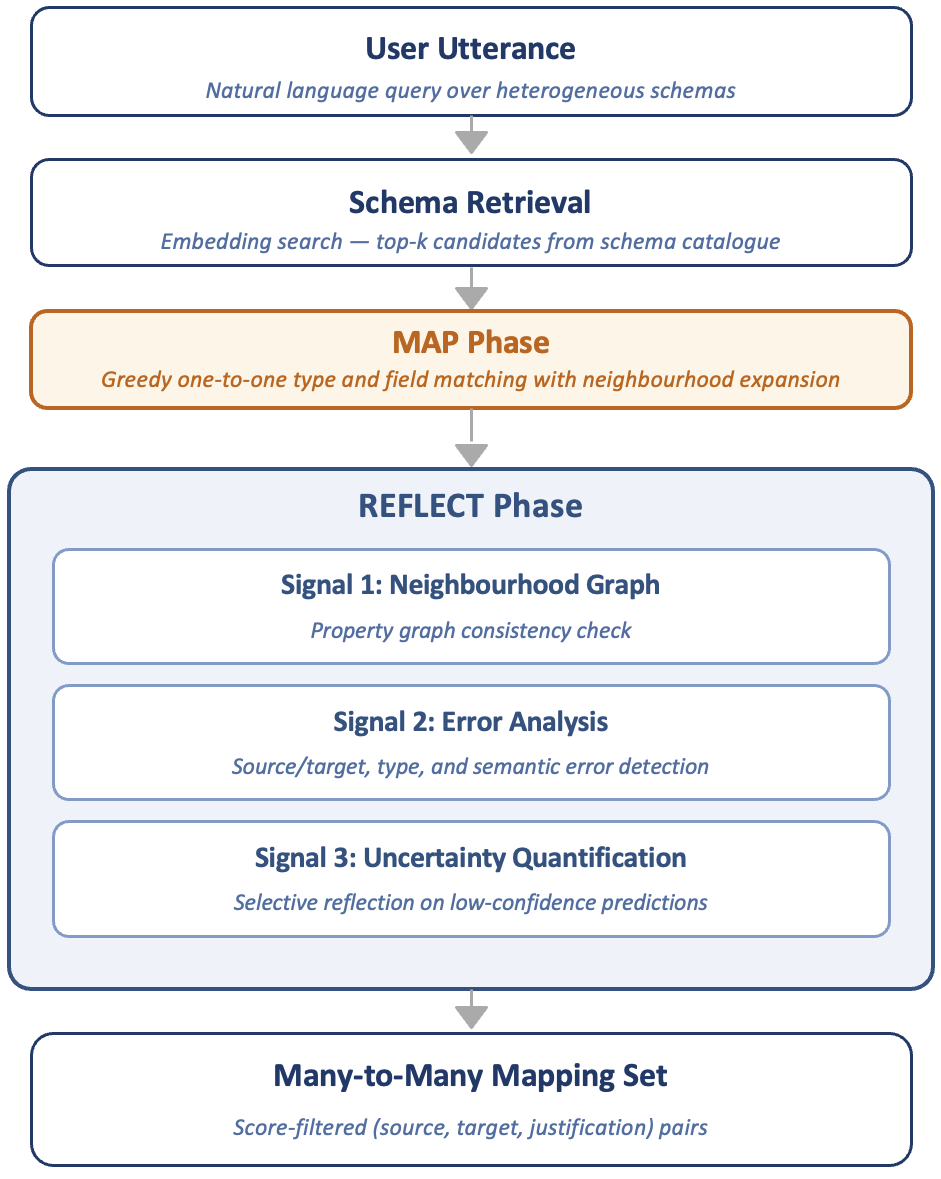
\includegraphics[width=0.7\columnwidth]{intro_diagram.png}
    \caption{Map-Reflect pipeline: greedy MAP followed by signal-driven REFLECT.}
    \Description{Map-Reflect pipeline showing User Utterance flowing through Schema Retrieval, MAP Phase, REFLECT Phase with three signals (Neighbourhood Graph, Error Analysis, Uncertainty Quantification), and outputting Many-to-Many Mapping Set.}
    \label{fig:pipeline}
\end{figure}

Traditional approaches focus on database integration with column-level mapping, but enterprise environments require schema retrieval and multi-faceted mapping across both APIs and databases. For example, Site Reliability Engineers managing hybrid cloud environments must query across multiple observability platforms, each with distinct schemas. Mapping across these disparate systems creates substantial overhead.

\paragraph{The Many-to-Many Challenge.}
Prior work on schema mapping focuses on one-to-one alignments~\cite{matchmaker, sheetrit2024rematch} or single-chain API sequencing~\cite{saha-etal-2024-sequential}. Real enterprise environments require \emph{many-to-many mappings} where multiple source types/fields correspond to overlapping target structures. For example, \texttt{Incident} from one system may correctly map to both \texttt{Alert} and \texttt{Event} in another. Greedy one-to-one mapping leaves too many elements unmapped, while naive approaches create spurious mappings that break query semantics. Many Large Language Models (LLM) based solutions for this problem use reflection. A key challenge for any reflection mechanism is knowing \emph{when} to reflect: firing unconditionally corrupts correct predictions, while a reliable trigger must identify genuinely uncertain cases. Uncertainty quantification provides this gate. As we show on diverse datasets, UQ-triggered reflection is the only trigger that does not reduce field recall; all other signals fire too broadly and over-correct predictions that were already correct.

Recent advances in tool calling with large language models show promise for API-related tasks. ToolLLM~\cite{toolllm} and AnyTool~\cite{anytool} focus on sequencing a single chain of calls; they do not address systematic alignment of schema elements across products, which is the prerequisite for variable mapping between function calls. Sequential function calling with variable mapping across APIs has been studied by~\citet{saha-etal-2024-sequential}, who introduce GraphQLRestBench and demonstrate that GraphQL schema representations are effective for encoding API response structure in LLM prompts for multi-step API sequencing. Self-reflection mechanisms in these approaches lack external grounding because the model critiques its own output without validation against external signals, potentially reinforcing errors~\cite{huang2024selfcorrect}. Further, AnyTool requires GPT-4, limiting practical applicability.

\paragraph{The Pre-processing Cost Problem.}
Schema inventories in enterprise deployments are never static: Data Fabric and Data Mesh implementations~\cite{blohm2024data,dehghani2022datamesh} grow through M\&A activity and SaaS onboarding; Backend for Frontend patterns~\cite{richardson2018microservices} require re-alignment every time a new upstream service is added; and agentic code tools such as Claude Code and Gemini CLI need schema mapping as a \emph{runtime} capability rather than a batch offline step. AnyTool~\cite{anytool} requires rebuilding a multi-vector index, a DSPy bootstrapping loop, and a three-tier agent hierarchy whenever schemas change, and reports 43.3 GPT-4 calls per query in its original setting. In our problem setting, we want to avoid such expensive pre-processing steps and also the dependence on frontier models.

Building a unified Data Access Layer (DAL) or a Common Data Model requires mapping schemas across both APIs and databases. Hence we evaluate on API datasets (ITOpsGraph, NL2GQL, ToolBench) and database schemas (OMOP, SchemaNet). Our ITOpsGraph benchmark provides schema mapping across heterogeneous enterprise APIs, featuring (i)~deeply nested type hierarchies, (ii)~domain-specific terminology where semantically equivalent concepts have different names, and (iii)~many-to-many mappings where a single source type correctly maps to multiple targets. Our wiki-based Subject Matter Expert (SME) annotation provides continuous ground truth refinement.

% FIX ISSUE_3: Added Mistral-Large-2 to the model list in the introduction
We introduce Map-Reflect, an \emph{gated reflection} framework that addresses the above limitations through a two-phase approach (Figure~\ref{fig:pipeline}). In the first \emph{Map} phase, we greedily find the best mapping for each source type and its fields. In the second \emph{Reflect} phase, we explore three candidate external signals to gate reflection: a \emph{neighbourhood graph} that validates mapping assumptions, \emph{error analysis} from schema deployment and query execution, and \emph{uncertainty quantification} that selectively targets genuinely ambiguous predictions. As the ablation in Section~\ref{sec:ablation} shows, only the UQ signal avoids degrading accuracy; the other two hurt by over-correcting correct predictions. Besides empirical evidence, we provide theoretical grounding for UQ as a reflection trigger based in the consistency hypothesis~\cite{xiao2025consistency} and SIMBA~\cite{simba2025}. Unlike AnyTool, which requires building a static GPT-4--driven three-tier hierarchy before any mapping can be performed, Map-Reflect operates with open-source models (Llama-3.3-70B, Mistral-Large-2, Granite-4-small) and additionally supports runtime target discovery from a live catalogue with no offline pre-processing.

Our contributions are as follows:
\begin{itemize}[noitemsep,topsep=2pt,leftmargin=*]
  \item \textbf{Map-Reflect}, a two-phase gated reflection framework for schema-agnostic, GPT-free schema mapping across REST APIs, GraphQL, and relational databases. A greedy Map phase produces an initial alignment; a UQ-gated Reflect phase refines it selectively. The framework supports runtime target discovery from a live catalogue with no offline preprocessing.
  \item \textbf{Empirical study of reflection triggers} for LLM-based schema mapping, showing that structural and heuristic signals degrade accuracy by firing on already-correct predictions, while only uncertainty-guided reflection avoids degradation across all evaluated benchmarks (Section~\ref{sec:ablation}).
  \item \textbf{ITOpsGraph benchmark}: the first enterprise API schema mapping benchmark spanning multiple schema paradigms (GraphQL and proto buffer), 12 products, 11,110 RAG-enriched fields, and human-validated ground truth covering many-to-many mappings across heterogeneous naming conventions.
  \item \textbf{ITOpsGraph-MB benchmark}: the first human-annotated many-to-many schema mapping benchmark with bipartite field constraints, covering 786 type pairs and 3,030 field mappings across 12 enterprise products (Section~\ref{sec:itgraph_mb}).
\end{itemize}


\section{Related Work}

Table~\ref{tab:method_comparison} positions Map-Reflect against prior methods across six capability dimensions. No existing method covers all six; Map-Reflect is the only system combining LLM reasoning, structural context, runtime reflection, relational schema mapping, API mapping, and many-to-many support.

\begin{table}[htbp]
\centering
\small
\caption{Method capability comparison across six dimensions.}
\label{tab:method_comparison}
\resizebox{\columnwidth}{!}{%
\begin{tabular}{l ccccc}
\toprule
\textbf{Method} & \textbf{LLM} & \textbf{Structural} & \textbf{Reflection} & \textbf{API} & \textbf{Many-to-} \\
 & & & & \textbf{Mapping} & \textbf{Many} \\
\midrule
COMA~\cite{10.5555/1287369.1287422}        & \texttimes & \checkmark & \texttimes & \texttimes & limited \\
Magneto~\cite{liu2024magneto}               & \checkmark & \texttimes & \texttimes & \texttimes & \texttimes \\
ReMatch~\cite{sheetrit2024rematch}          & \checkmark & \texttimes & \texttimes & \texttimes & \texttimes \\
LLMatch~\cite{wang2025llmatch}              & \checkmark & \texttimes & \texttimes & \texttimes & \checkmark \\
MatchMaker~\cite{matchmaker}                & \checkmark & \texttimes & \texttimes & \texttimes & \texttimes \\
AnyTool~\cite{anytool}                      & \checkmark & \texttimes & \checkmark & \checkmark & \texttimes \\
\midrule
\textbf{Map-Reflect (ours)}                 & \checkmark & \checkmark & \checkmark & \checkmark & \checkmark \\
\bottomrule
\end{tabular}
}
\end{table}

\paragraph{Classical Schema Matching.} Early schema mapping systems include Clio~\cite{miller2001clio,fagin2009clio}, which pioneered automated schema mapping and data exchange, and LSD~\cite{doan2003learning}, which applied machine learning to ontology mapping. Cupid~\cite{madhavan2001generic}, COMA/COMA++~\cite{10.5555/1287369.1287422,ahn2005comapp}, and iMAP~\cite{dhamankar2004imap} combine linguistic, structural, and domain-specific similarity~\cite{rahm2001survey,euzenat2013ontology}. Similarity Flooding~\cite{melnik2002similarity} propagates similarity scores across schema graphs using fixpoint computation. Bernstein et al.~\cite{bernstein2011generic} survey a decade of progress and identify many-to-many mapping and schema heterogeneity as persistent open problems. The Ontology Alignment Evaluation Initiative~\cite{euzenat2011ontology} provides standardised benchmarks; Valentine~\cite{koutras2021valentine} extends these to tabular data. All classical systems assume flat relational schemas with one-to-one correspondences. DynaMap~\cite{mazilu2022schema} and SMUTF~\cite{zhang2025smutf} add dynamic programming and gradient-boosted classifiers but still lack semantic reasoning. API retrieval and sequencing have been addressed by embedding-based retrievers~\cite{li2023api,patil2023gorilla}, fine-tuned methods~\cite{toolllm}, graph-based approaches~\cite{mandal2024graph}, and GraphQL-based sequential function calling~\cite{saha-etal-2024-sequential}.

\paragraph{Learning-Based Matching.} Neural approaches brought deep learning to entity and schema matching. Magellan~\cite{konda2016magellan} provides infrastructure for building entity matching pipelines using feature engineering. DeepMatcher~\cite{mudgal2018deep} systematically explores deep learning architectures for entity matching; Ditto~\cite{li2020ditto} applies pre-trained transformers~\cite{vaswani2017attention,devlin2019bert} to achieve strong pairwise attribute matching. Trabelsi et al.~\cite{trabelsi2019schema} extend BERT to schema matching tasks, and Thirumuruganathan et al.~\cite{thirumuruganathan2020deep} survey the design space. Toolformer~\cite{schick2023toolformer} shows that LLMs can learn to invoke tools via self-supervised training, motivating API-schema mapping as a structured reasoning task. These methods focus on pairwise correspondences and do not exploit structural dependencies across schema graphs.

\paragraph{LLM-Based Schema Mapping.} The emergence of large language models~\cite{brown2020language,ouyang2022training} enabled a new generation of schema matching systems that leverage semantic understanding from pre-training. LSM~\cite{zhang2023schema} uses fine-tuned BERT encoders; Magneto~\cite{liu2024magneto} combines SLMs with LLM reranking; ReMatch~\cite{sheetrit2024rematch} and GraphRAGToolFusion~\cite{lumer2025graphragtoolfusion} add retrieval. MatchMaker~\cite{matchmaker} introduced compositional LLM programs with offline DSPy~\cite{khattab2023dspy} bootstrapping, but targets only flat relational schemas and requires ColBERT-v2 indexing before deployment. LLMatch~\cite{wang2025llmatch} adds Rollup/Drilldown for many-to-many relational matching; SCHEMORA~\cite{gungor2025schemora} uses BM25 and FAISS~\cite{johnson2019billion} retrieval but requires upfront column-group normalization that assumes SQL tabular input, inapplicable to nested API schemas. Reflection-based LLM agents including ReAct~\cite{yao2023react}, Reflexion~\cite{shinn2023reflexion}, and chain-of-thought reasoning~\cite{wei2022chain} demonstrate that iterative self-revision improves structured reasoning, but rely on unconditional reflection without external grounding signals — a limitation our ablation quantifies. AnyTool~\cite{anytool} applies GPT-4~\cite{achiam2023gpt4} function calling with a static three-tier API hierarchy — effective for tool sequencing but not schema mapping, and not transferable without rebuilding the taxonomy.

\paragraph{Uncertainty Quantification for LLMs.}
Black-box UQ methods rely only on model outputs and are compatible with proprietary APIs~\cite{xiao2025consistency,simba2025}. Self-consistency~\cite{wang2023selfconsistency} showed that sampling multiple chain-of-thought paths and taking the majority improves reasoning accuracy — an early demonstration that generation agreement signals correctness. Subsequent work formalised this as a proxy for hallucination detection~\cite{lin2024generating,manakul2023selfcheck}. The consistency hypothesis~\cite{xiao2025consistency} generalises this: correct LLM generations are more similar to each other than incorrect ones, an effect strongest on structured-output tasks including text-to-SQL. SIMBA~\cite{simba2025} generalises this as a family of similarity-based aggregation functions; classification over pairwise similarities yields the best-calibrated estimates for structured outputs. Map-Reflect's UQ gate is grounded in this framework: entropy over MAP-phase candidate confidences identifies genuinely ambiguous predictions and selectively triggers reflection only for those fields.


\section{Map-Reflect Framework}
\label{sec:mapreflect}

Our two-phase architecture is designed for the many-to-many mapping challenge. Map-Reflect is schema-agnostic: it handles REST APIs, GraphQL, and relational databases uniformly, operating at two levels regardless of schema paradigm. \textbf{Type-level mapping} identifies semantically equivalent entities — GraphQL types, REST resources, or database tables (e.g., \texttt{VirtualMachine} in one system maps to \texttt{EC2Instance} in another). \textbf{Field-level mapping} aligns constituent attributes within mapped type pairs — GraphQL fields, REST parameters, or database columns. The first phase (Map) performs greedy one-to-one mapping, which is fast but leaves many elements unmapped and may create spurious mappings. The second phase (Reflect) explores three candidate external signals for gated reflection: neighbourhood graph validation, error analysis, and uncertainty quantification. As the ablation in Section~\ref{sec:ablation} establishes, only UQ-triggered reflection should be used by default. Given API specifications or database schemas, Map-Reflect applies the two-phase mapping process.

New schemas require only parsing and optional RAG enrichment — no graph construction, model training, or offline preprocessing. This makes Map-Reflect practical for the live-catalogue target discovery setting (Section~\ref{sec:retrieval_results}), where new APIs are registered continuously and a static hierarchy would require rebuilding.

Unlike GPT-4-centric tool agents, our components are invoked but never trained. A user utterance $u$ is processed in five stages. First, a context extractor splits $u$ into source and destination phrases by prompting a hosted chat model. Second, each phrase is embedded and queried against a Chroma vector index, yielding neighbourhoods $\mathcal{S}_{\mathrm{src}}$ and $\mathcal{S}_{\mathrm{dst}}$. Third, a reasoning call evaluates every pair in $\mathcal{S}_{\mathrm{src}}\times\mathcal{S}_{\mathrm{dst}}$, assigns a confidence $\gamma_0$, and produces justifications; this is the greedy Map phase. Fourth, the Reflect phase collects three external signals and induces reflection to refine mappings. Finally, mappings with scores below threshold $\tau_p$ are pruned, yielding many-to-many coverage. When the evaluation utterance already names both source and target schemas directly, the context extractor step is bypassed; the full five-stage pipeline applies in the runtime target discovery setting (Section~\ref{sec:retrieval_results}).

\subsection{Two-Phase Architecture: Map and Reflect}

\textbf{Phase 1: Map (Greedy One-to-One).} For each source type $T_s$ in the source schema, we compute embedding similarity with all types in the target schema and select the highest-scoring target type $T_t$ as the initial mapping. For each field $F_s$ in the mapped source type, we similarly select the best matching field $F_t$. This produces a fast one-to-one mapping with confidence scores, but leaves many types/fields unmapped and may create spurious mappings based on superficial similarity.

\textbf{Phase 2: Reflect (Uncertainty-Guided Refinement).} The Reflect phase selectively refines the greedy mapping using external signals: \emph{coverage analysis} identifies unmapped source and target elements, \emph{signal collection} gathers neighbourhood validation, error analysis, and uncertainty scores, \emph{gated reflection} explores alternative mapping targets for high-uncertainty elements, and \emph{spurious mapping removal} verifies one-to-many mappings and removes those that fail validation. Our ablation (Section~\ref{sec:ablation}) shows that of the three signals, only UQ-triggered reflection avoids degrading accuracy; error-based and neighbourhood-based signals fire too broadly, over-correct correct predictions, and are not recommended in the default configuration.

\subsection{Gated Reflection Mechanism}

Induced reflection refines mappings using external signals rather than model self-critique alone (Figure~\ref{fig:reflection_example}). We explore three external signals:

\begin{figure*}[t]
    \centering
    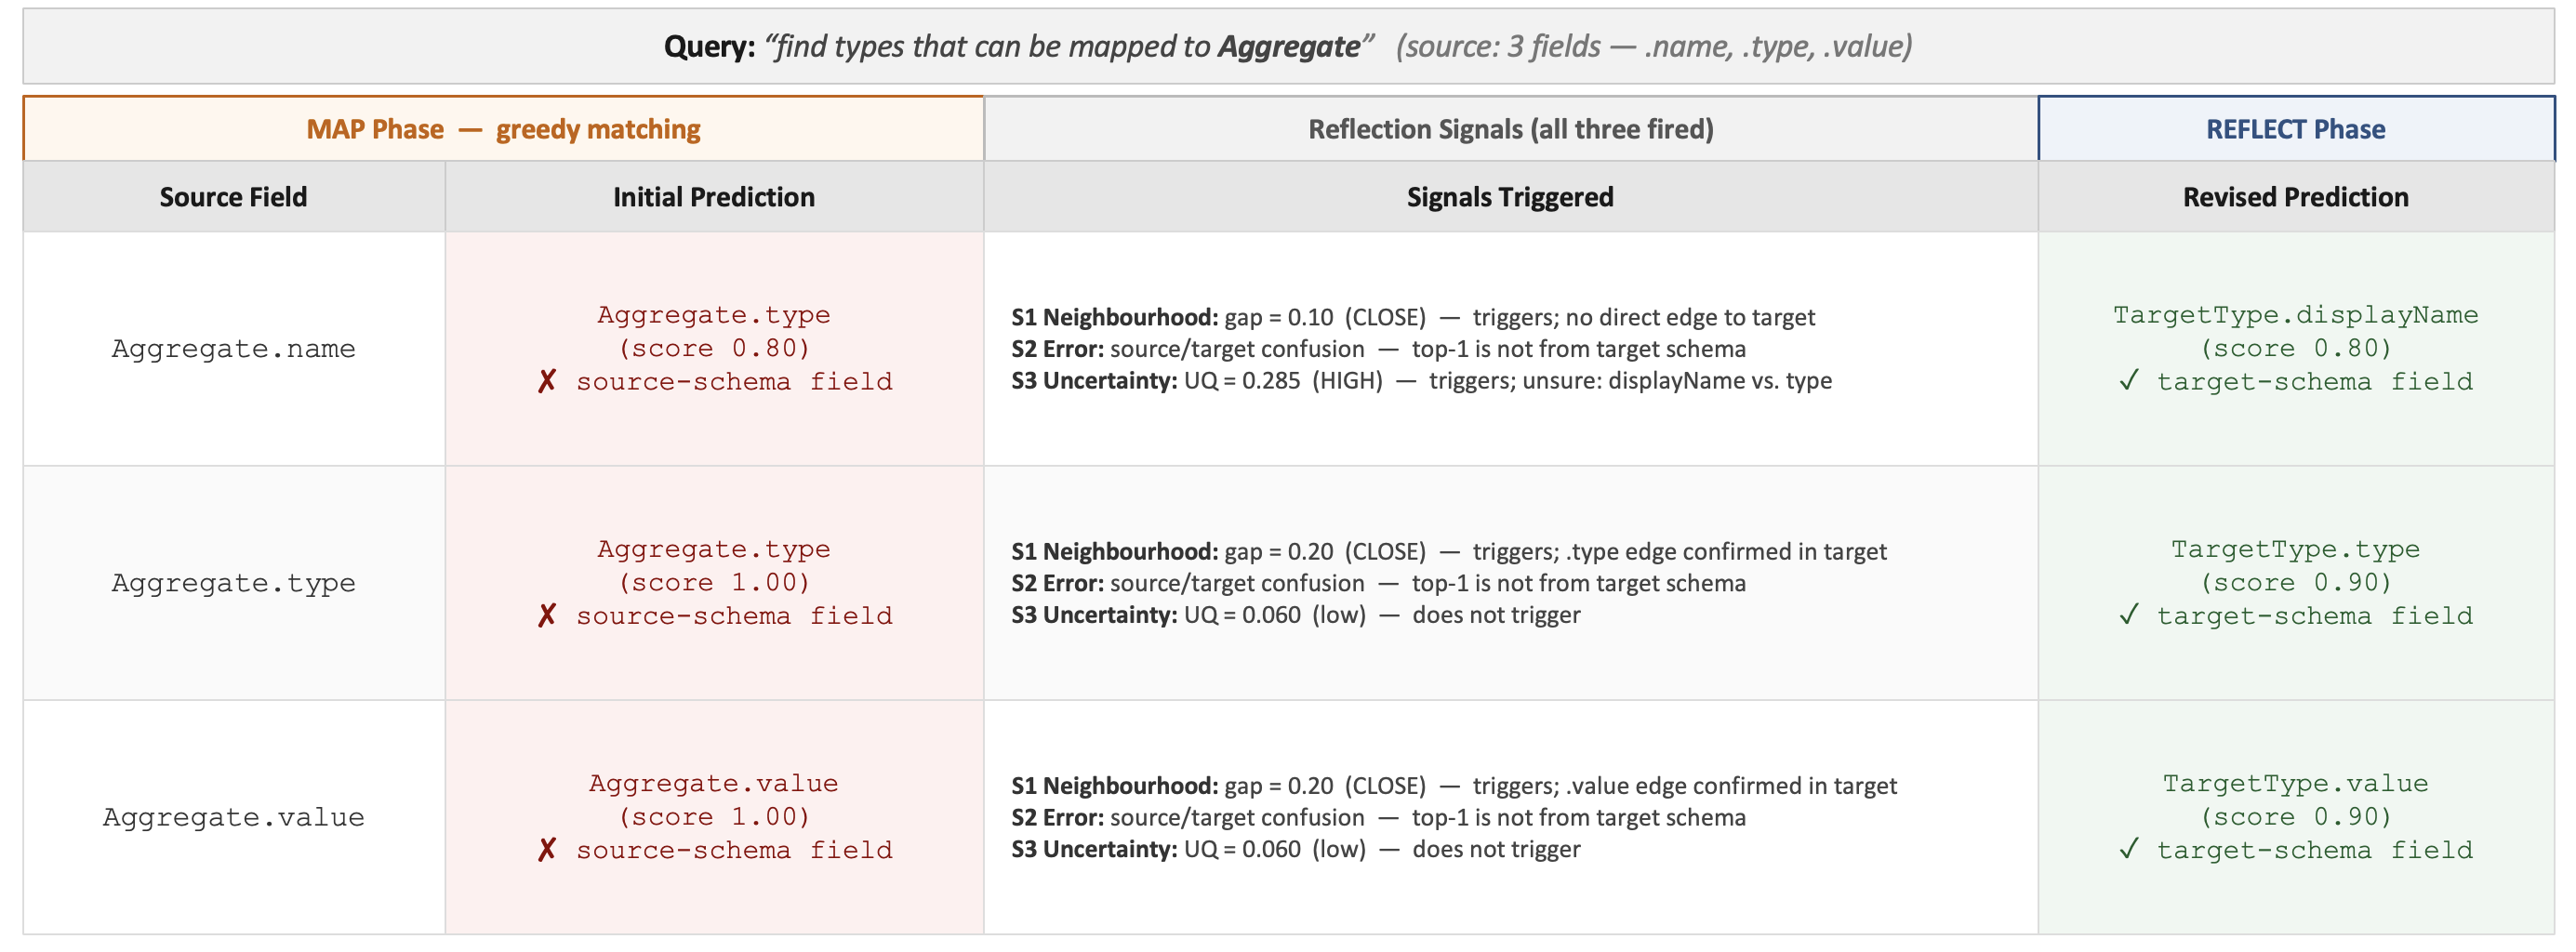
\includegraphics[width=\textwidth]{solution_diagram.png}
    \caption{Gated reflection on ITOpsGraph. MAP phase produces incorrect predictions; three external signals trigger reflection; REFLECT phase corrects to target-schema fields with improved confidence.}
    \Description{Map-Reflect correction: three source fields, wrong initial predictions, reflection signals, revised correct predictions.}
    \label{fig:reflection_example}
\end{figure*}

\textbf{Signal 1: Neighbourhood Graph Validation.} For each candidate mapping $(s, t)$, we retrieve $k$-nearest neighbours from the graph store and validate whether neighbours of the source type also map to neighbours of the target type, whether alternative targets with similar structure exist, and whether any unmapped neighbours should be included. The neighbourhood consistency gap $g = 1 - |\mathcal{N}_k(s) \cap \mathcal{N}_k(t)| / |\mathcal{N}_k(s)|$ quantifies this; when $g > 0.2$, the signal fires. If neighbourhood evidence contradicts the greedy mapping, we add alternative mappings (achieving many-to-many coverage) or remove inconsistent ones.

\textbf{Signal 2: Error Analysis.} Before reflection, we analyse the greedy mapping's ranking for structural error patterns: product mismatch (source and target belong to different product namespaces), foreign key misalignment (join keys are incompatible), low confidence (top candidate score $< 0.5$), and ambiguous top-2 predictions (score gap $< 0.1$). We also attempt to deploy a unified schema, surfacing type conflicts and null query results. Detected patterns are passed as structured context to the reflection prompt.

\textbf{Signal 3: Uncertainty Quantification.}
Let the MAP phase return $n \leq 20$ ranked candidates for source field $f$ (top-$k$=10 retrieved; up to 20 sent to the LLM), with LLM-assigned scores $\gamma_j \in [0,1]$ per candidate. These are raw scores assigned independently by the LLM and do not form a probability distribution. We compute a weighted uncertainty score
\begin{equation*}
u(f) = 0.3(1-\gamma_1) + 0.3(1 - \Delta\gamma) + 0.2\,\mathbb{1}[\text{no reasons}] + 0.06,
\end{equation*}
where $\gamma_1$ is the top-candidate score, $\Delta\gamma = \max_j \gamma_j - \min_j \gamma_j$ is the score range across all ranked candidates, and $\mathbb{1}[\text{no reasons}]$ is 1 when the LLM returns no supporting reasoning for its top prediction. The three terms capture: (i) low confidence in the top candidate, (ii) low discrimination between candidates (clustered scores indicate ambiguity), and (iii) absence of grounded justification. We trigger reflection when $u(f) > \tau_u = 0.25$.

This is a single-pass proxy for the generation-consistency signal in SIMBA~\cite{simba2025}, approximating the low-consistency regime where predictions are most likely wrong. We validated the proxy on ITOpsGraph: the heuristic gate fires on 58 fields while the sampling-based SIMBA gate (three stochastic passes at temperature~0.7) fires on 61 fields, confirming near-identical coverage and that the proxy identifies the same uncertain predictions without repeated inference. Empirical calibration further validates the gate: fields above $\tau_u$ have 20\% MAP accuracy versus 84\% for fields below it, and accuracy decreases monotonically across uncertainty quartiles (Q1: 95\%, Q2: 80\%, Q3: 68\%, Q4: 60\%).

\begin{figure}[htbp]
    \centering
    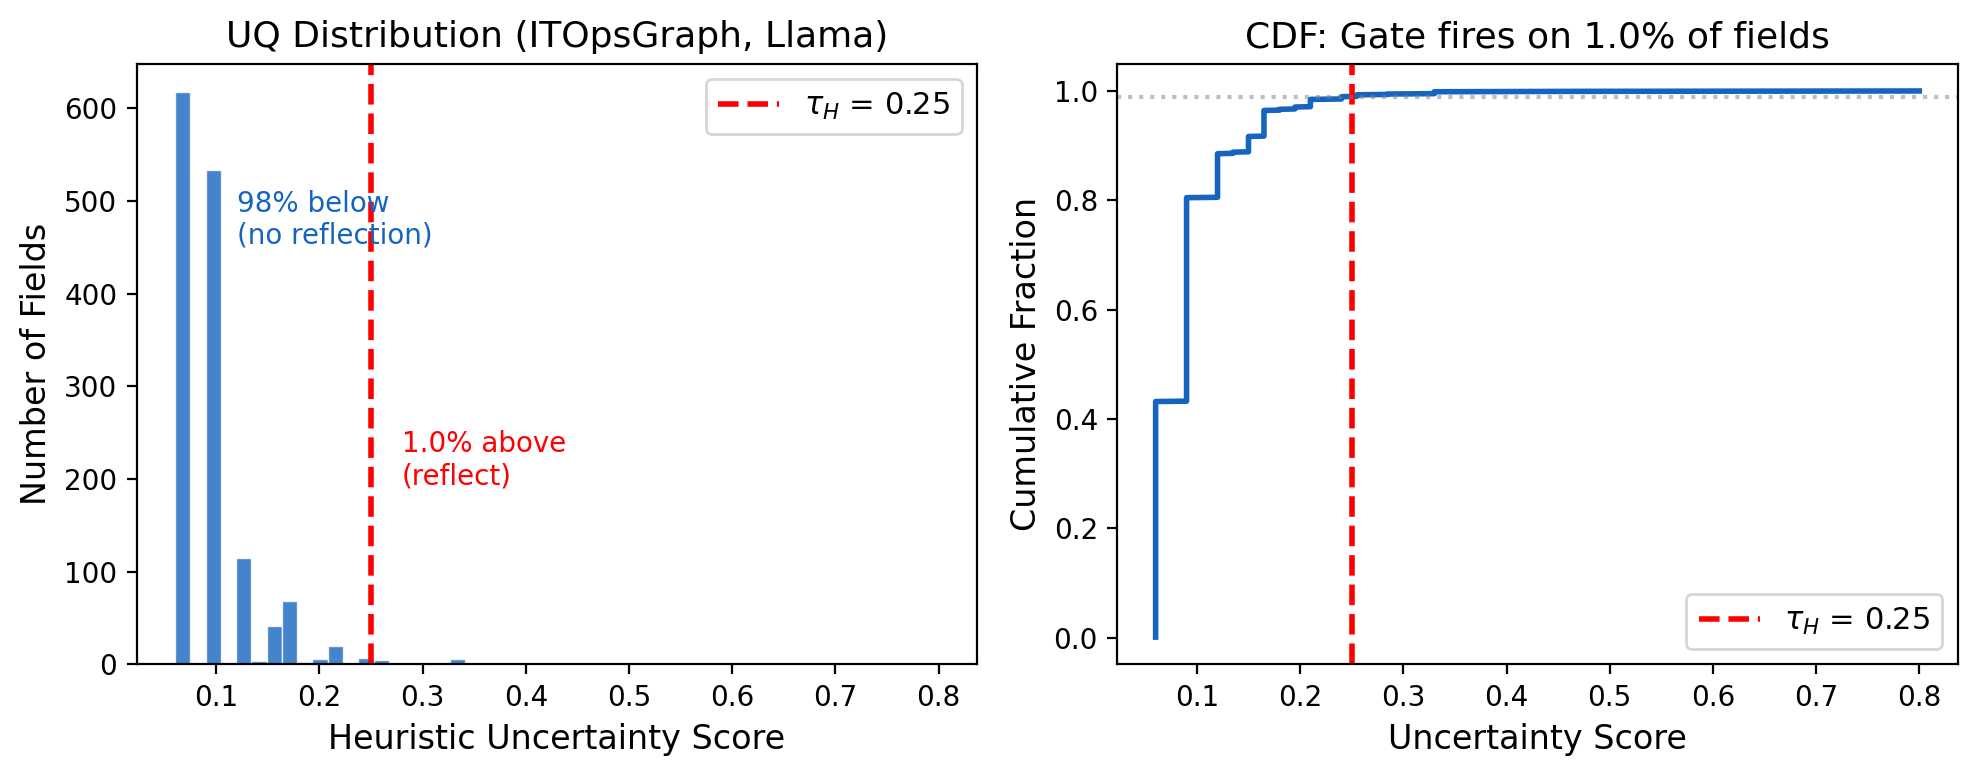
\includegraphics[width=\columnwidth]{chart_entropy_distribution.png}
    \caption{MAP-phase UQ score distribution on ITOpsGraph (1,429 fields, Llama-3.3-70B). The gate fires on only 1.0\% of fields (those above $\tau_u = 0.25$); the bulk of the distribution is well below the threshold, confirming robustness.}
    \label{fig:entropy_dist}
\end{figure}

Let $\gamma_r(s,t)$ be the confidence after reflection round $r$. Scores are updated as
\begin{equation}
\gamma_{r+1}(s,t)=\operatorname{clip}(\gamma_r(s,t)+\eta\,\Delta_r(s,t),0,1),
\label{eq:update}
\end{equation}
where $\eta{=}0.1$. $\Delta_r(s,t)\in[-1,0]$ is non-positive: signals apply only penalties, not boosts, since external evidence can disconfirm a mapping but cannot independently confirm one (confirmation comes from the LLM ranking itself). The neighbourhood signal sets $\Delta_r = -(g - 0.2)$ when gap $g = 1 - |\mathcal{N}_k(s) \cap \mathcal{N}_k(t)| / |\mathcal{N}_k(s)|$ exceeds 0.2; the error signal sums per-error penalties ($-0.40$ to $-0.10$); the UQ signal sets $\Delta_r = -(u(f) - \tau_u)$.

\textbf{Replacement path.} When a penalised score falls below $\tau_p{=}0.5$, the mapping $(s,t)$ is replaced by the next-highest-scoring alternative from the MAP-phase ranked list, which inherits that candidate's MAP score $\gamma_1$. A fresh MAP call is issued if the ranked list is exhausted.

\textbf{Many-to-many addition path.} This is logically distinct from replacement. After replacement is resolved, the neighbourhood signal checks whether neighbours of $s$ map to targets not yet assigned to $s$. Any such target $t'$ is scored by a fresh MAP call; if its score exceeds $\tau_p$, the pair $(s, t')$ is \emph{added} to the output alongside $(s,t)$, producing many-to-many coverage. Many-to-many additions therefore arise from positive neighbourhood evidence, not from the penalty-only score update equation, which only governs whether existing mappings survive pruning.

\section{ITOpsGraph Benchmark}
\label{sec:itopsgraph}

Existing schema mapping benchmarks focus on flat relational schemas
(OMOP, SchemaNet) or single-domain API corpora (ToolBench, NL2GQL).
None expose the combination of challenges that characterise real
enterprise integration: heterogeneous schema paradigms, deeply nested
type hierarchies, domain-specific terminology where semantically
equivalent concepts carry entirely different names across products,
and legitimate many-to-many mappings where a single source type
correctly aligns with multiple targets.
We introduce \textbf{ITOpsGraph}, an enterprise API schema mapping
benchmark built from production IT operations and cloud infrastructure
schemas, and \textbf{ITOpsGraph-MB}, a derived many-to-many mapping
benchmark with human-annotated bipartite field correspondences.
Both datasets and the annotation tooling are released at
\url{https://github.com/balajinix/map-reflect}.

\subsection{Schema Collection and Enrichment}

ITOpsGraph is built from two families of production schemas spanning
12 products across IT operations and cloud infrastructure:

\textbf{Observability products (GraphQL).}
We parse GraphQL SDL~\cite{graphql2021spec} from six products:
Instana (infrastructure monitoring), Turbonomic (resource optimisation),
Concert (AIOps platform), Cloudability (cloud cost management),
NS1 (DNS and traffic management), and Watsonx-Orchestrate (AI
workflow automation). GraphQL schemas expose deeply nested type
hierarchies with interface inheritance and union types.

\textbf{Cloud infrastructure tools (proto buffer).}
We parse Protocol Buffer~\cite{google2023protobuf} definitions from
five tools: AWS, Azure, and GCP cloud provider schemas, HashiCorp
Terraform (infrastructure-as-code), and HashiCorp Packer (image
building). Proto buffer schemas use flat repeated fields where
GraphQL uses nested objects, creating paradigm-boundary challenges
for cross-system mapping.

Parsing yields 1,640 types and 10,876 fields across the 12 products.
To enrich field descriptions, we convert 239\,MB of product
documentation (PDF manuals and API references) using
docling~\cite{auer2024docling} and index the resulting text in
ChromaDB~\cite{chromadb2023}. For each field, we retrieve the
three most relevant documentation passages and concatenate them
as a RAG-enriched~\cite{lewis2020retrieval} description. This
process surfaces an additional 234 fields referenced in
documentation but absent from the parsed schemas, bringing the
total to \textbf{1,640 types and 11,110 RAG-enriched field
descriptions}. The unified schema is loaded into a typed property
graph (Section~\ref{sec:nbr_graph}) and served through a
vector index (Milvus~\cite{wang2021milvus}) for retrieval.

\subsection{Neighbourhood Graph}
\label{sec:nbr_graph}

The neighbourhood graph is a property graph over the unified schema
that enables structure-aware candidate expansion during mapping.
We construct it using NetworkX~\cite{hagberg2008networkx} with three
weighted edge types:
same-type edges (weight 0.3) connect all fields within the same type;
cross-type edges (weight 0.7) connect fields across types within the
same product; and semantic edges connect fields across products when
their embedding similarity exceeds 0.8, weighted by the similarity score.
Each node carries four attributes: fully qualified name, parent type,
source product, and RAG-enriched description.

During the Map phase, after retrieving initial candidates via
dense-vector search, we expand the candidate set by traversing
$k{=}5$ hops from each retrieved candidate (chosen by grid search
over $\{2,3,5,7\}$ on a held-out validation split).
Neighbours are added to the candidate pool weighted by path distance,
surfacing semantically related fields that embedding similarity over
short identifier strings alone would miss.
Graph construction for the full 11,110-field schema takes
approximately 80 seconds on commodity hardware and is persisted
across mapping sessions.
During the Reflect phase, the graph is additionally queried to
validate neighbourhood consistency: if \texttt{TypeA} maps to
\texttt{TypeB}, neighbours of \texttt{TypeA} should also map to
neighbours of \texttt{TypeB}.

\subsection{Wiki-Based Schema Documentation}

We deploy a MediaWiki~\cite{mediawiki} instance organised hierarchically
by product, type, and field. Each product has a dedicated page
documenting its schema structure; type pages list constituent fields
with descriptions and usage notes; and bidirectional hyperlinks connect
semantically equivalent fields across products. The wiki currently
documents all 12 products, 1,679 types, and 11,110 field descriptions
with RAG-enhanced content. It serves two roles: a living documentation
resource that evolves as products change, and the interface through which
subject matter experts (SMEs) review candidate mappings before they are
promoted to ground truth.

\subsection{Human Annotation}
\label{sec:annotation}

Ground truth for both benchmarks is produced through a purpose-built Streamlit annotation tool that presents each candidate type pair alongside field mappings from an ensemble of seven schema mapping methods with per-method confidence scores, and RAG-enriched field metadata. For each type pair the annotator assigns a type-level judgment (\emph{Correct}, \emph{Plausible}, \emph{Incorrect}, or \emph{Uncertain}) and accepts, rejects, or corrects each candidate field mapping. The tool enforces the bipartite constraint in real time: once a target field is assigned, it is removed from the dropdown for remaining source fields. Annotations are saved incrementally as JSONL with full provenance.

The ensemble methods serve solely as candidates to reduce cold-start effort; the annotator makes all authoritative decisions independently. Ground truth was produced by a single domain expert with deep knowledge of all 12 products; formal inter-annotator agreement was not measured, which is a limitation. Three design choices mitigate annotation bias: (i) the ensemble shows disagreement across seven methods, discouraging anchoring on any single system's output; (ii) the bipartite constraint is enforced mechanically rather than judgmentally, removing discretion from the most consequential field-level decisions; and (iii) all accept/reject/correct decisions are logged with timestamps, enabling post-hoc audit. For ITOpsGraph-MB, pairs where the annotator marked the type judgment as \emph{Uncertain} are excluded from the evaluation set.

\subsection{One-to-One Evaluation}

ITOpsGraph contains \textbf{521 evaluation samples} representing cross-product type mapping tasks, each pairing a source type from one product with a target type from another, with human-validated field-level ground truth. The benchmark poses three challenges: \textbf{schema paradigm heterogeneity}, where GraphQL nested object types become flat repeated fields in proto buffer; \textbf{domain-specific terminology}, where semantically equivalent fields carry entirely different names (\texttt{severity} vs \texttt{criticalityLevel}, \texttt{Alert} vs \texttt{Incident}); and \textbf{legitimate many-to-one mappings}, where multiple source fields correctly map to the same target field when a standardised schema consolidates proprietary fields.

\subsection{Many-to-Many and Bipartite}
\label{sec:itgraph_mb}

ITOpsGraph-MB evaluates the harder setting where one source API type
legitimately maps to multiple target types, and within each type pair
field mappings are bipartite: each target field is claimed by at most
one source field.
We first generate candidate type pairs by running an ensemble of seven
schema mapping systems on all cross-product type pairs across the 12
products, retaining pairs predicted by at least two method/model
combinations with at least two candidate bipartite field mappings.
All retained pairs are then validated through the human annotation
workflow (Section~\ref{sec:annotation}): the annotator reviews each
type pair, assigns a type-level judgment, and accepts, rejects, or
corrects each field mapping with the bipartite constraint enforced live.

The resulting \textbf{ITOpsGraph-MB} benchmark contains 786 human-validated
type pairs with 3,030 bipartite field mappings across 12 products.
To our knowledge, it is the first human-annotated benchmark for
many-to-many schema mapping with bipartite field constraints on
enterprise API schemas. Existing many-to-many benchmarks (SchemaNet,
SCHEMORA) target flat relational schemas with primary/foreign key
annotations; none span multiple schema paradigms or require expert
judgment on cross-product naming divergence at this scale.

A GNN baseline trained on the full ITOpsGraph-MB graph (1,148 type pairs,
12,879 nodes) using GraphSAGE~\cite{hamilton2017inductive} with link
prediction provides a structural upper bound for comparison.

\section{Experiments}

We compare Map-Reflect against three baseline approaches. The \textbf{GNN} baseline uses a two-layer Graph Convolutional Network~\cite{kipf2017gcn} with 128-dimensional embeddings trained on ITOpsGraph pairs and evaluated zero-shot on all other datasets, except Spider where a separate GNN is trained on the Spider FK graph (Section~\ref{sec:results}). \textbf{AnyTool}~\cite{anytool} represents hierarchical retrieval with self-reflection via a static GPT-4--driven three-tier taxonomy; we re-implement with Llama-3.3-70B and evaluate with oracle-mode utterances naming both source and target schemas explicitly. This matched-backbone policy isolates methodological differences from backbone effects. AnyTool with GPT-4 would likely score higher than our reported numbers, particularly on SchemaNet where it already leads — meaning our wins on the other six benchmarks are conservative lower bounds on the true methodological advantage of Map-Reflect over AnyTool's approach. \textbf{MatchMaker}~\cite{matchmaker} is a compositional LM program with zero-shot self-improvement via ColBERT-v2 retrieval and DSPy bootstrapping; it requires two offline preprocessing steps before deployment and evaluates only on flat relational schemas in its original paper. In the ablation, the configuration using only the UQ trigger corresponds to the recommended default.

Map-Reflect uses ChromaDB~\cite{chromadb2023} with sentence-transformer embeddings (\texttt{all-MiniLM-L6-v2}~\cite{reimers2019sentence}) for vector indexing and LLM calls via WatsonX~\cite{ibm2023watsonx} for core mapping logic. The UQ threshold is fixed at $\tau_u = 0.25$ with no dataset-specific tuning. All LLM calls use temperature~0 and a fixed random seed (42) for reproducibility.

We evaluate all methods using three LLMs: \textbf{Granite-4}
(\texttt{ibm/granite-4-h-small})~\cite{granite2025}, a smaller open-source model;
\textbf{Llama-3.3-70B} (\texttt{meta-llama/llama-3-3-70b-instruct})~\cite{grattafiori2024llama3},
providing stronger reasoning; and \textbf{Mistral Medium 25.05}
(\texttt{mistralai/mistral-medium-2505}), a large open-weights model.
All models are accessed via WatsonX~\cite{ibm2023watsonx}.
In the tables, ``Granite'' refers to Granite-4, ``Llama'' refers to Llama-3.3-70B,
and ``Mistral'' refers to Mistral Medium 25.05.
For fair comparison, all LLM-based baselines use the same model versions; the original AnyTool paper~\cite{anytool} used GPT-4, but we re-implement with Llama-3.3-70B to isolate methodological differences. MatchMaker also uses ColBERT-v2~\cite{colbert} (\texttt{colbert-ir/colbertv2.0}) for candidate retrieval and is evaluated with Llama-3.3-70B and Granite-4 backbones.

\subsection{Datasets}

We evaluate Map-Reflect on API and database schema mapping datasets representing diverse real-world scenarios:

\textbf{ITOpsGraph and ITOpsGraph-MB}: Enterprise API schema mapping benchmarks introduced in Section~\ref{sec:itopsgraph}. ITOpsGraph (Section~\ref{sec:itopsgraph}, §\emph{One-to-One Evaluation}) contains 521 evaluation samples across 12 products with human-validated field-level ground truth. ITOpsGraph-MB (Section~\ref{sec:itgraph_mb}) extends this to 786 many-to-many type pairs with 3,030 human-annotated bipartite field mappings.

\textbf{ToolBench Dataset}: We utilize the ToolBench dataset containing 49,937 REST APIs across 10,388 tools spanning 50 categories. For evaluation, we process the first 10,000 training queries and retain the 3,190 queries that involve at least two distinct APIs with overlapping parameter types. Queries involving only a single API are excluded.

\textbf{NL2GQL Dataset}~\cite{kesarwani-etal-2024-graphql}: Natural language to GraphQL API schema mapping dataset featuring e-commerce, social media, and content management system schemas. The dataset contains 437 mapping instances with varying complexity levels from simple field mappings to complex relationship transformations, testing systems' ability to handle domain-specific terminology across 54 GraphQL API schemas. NL2GQL is the only benchmark in our evaluation where the source is a natural language utterance rather than a schema element, making it the strongest test of schema-agnostic generalisation.

\textbf{OMOP Datasets}: We evaluate on three healthcare database schema mapping benchmarks derived from the OMOP Common Data Model~\cite{omop,garza2016omop,hripcsak2015ohdsi}: (i) \textbf{CMS} (Centers for Medicare \& Medicaid Services claims data), (ii) \textbf{MIMIC}~\cite{johnson2016mimic} (Medical Information Mart for Intensive Care), and (iii) \textbf{Synthea}~\cite{walonoski2018synthea} (synthetic patient data). These datasets test mapping between proprietary healthcare data formats and the standardized OMOP schema, featuring challenges such as vocabulary mapping (ICD codes~\cite{who2019icd10} to SNOMED~\cite{snomed2021}), temporal alignment, and cardinality differences. Unlike API mapping, database schema mapping involves relational constraints and referential integrity.

\textit{Ground Truth Protocol.} The OMOP ground truth mappings are derived from the OMAP benchmark~\cite{matchmaker}, which provides expert-curated field-level correspondences between source schemas (CMS, MIMIC, Synthea) and the OMOP CDM target schema. We follow the evaluation protocol of prior work~\cite{matchmaker}: evaluation utterances specify both source and target schemas (e.g., ``map MIMIC PATIENTS to OMOP PERSON''), reflecting the typical use case where healthcare organizations know they want to map their proprietary data to the OMOP standard. Since OMOP is the single standardized target, target discovery is not needed for these benchmarks.

\textbf{Spider Dataset}~\cite{yu2018spider}: We derive a schema mapping benchmark from Spider~1.0, a text-to-SQL dataset containing 166~databases with expert-defined foreign key relationships. Each foreign key defines a joinable column pair between two tables; we extract all 745~unique table pairs (793~field-level mappings) across 164~databases as evaluation samples. Unlike other benchmarks that provide mapping utterances, Spider's ground truth is structural (foreign keys), testing whether methods can discover joinability from schema structure alone. The mapping utterance is generated as ``map~\texttt{<source\_table>}~data to~\texttt{<target\_table>}~data.'' Spider is the largest and most diverse relational benchmark in our evaluation, spanning domains including music, flights, pets, cars, healthcare, and education.

\textbf{SchemaNet Dataset}~\cite{wang2025llmatch}: A relational database schema matching benchmark covering seven schema pairs of varying complexity (377 total mappings): bank1\_bank2, imdb\_sakila, and five OMOP target pairs (cms\_omop, mimic\_iii\_omop, synthea\_omop, cprd\_gold\_omop, cprd\_aurum\_omop~\cite{herrett2015cprd}). The OMOP pairs overlap structurally with our OMOP evaluation but use different source schemas and ground truth; results are therefore reported separately. SchemaNet tests purely relational schema alignment without API or graph paradigms, providing complementary coverage to the API-focused benchmarks.

Table~\ref{tab:eval_sizes} reports evaluation sample counts per dataset. Several reported accuracies approach saturation, which reflects structural properties of specific benchmarks rather than inflated methodology. OMOP type accuracy is 100\% because OMOP CDM is the single fixed target schema — there is no type discovery problem, only field mapping; the challenge is in Tables~\ref{tab:type_results}--\ref{tab:field_results}'s field F1 column. NL2GQL and ToolBench retrieval accuracy approaches saturation because GraphQL schema names are highly distinctive (54 schemas with domain-specific naming), making target retrieval tractable; the harder sub-problem is field-level mapping within the retrieved schema. These saturated settings are included for completeness and because they confirm schema-agnostic coverage, not to inflate overall performance claims.

\begin{table}[htbp]
\centering
\small
\caption{Evaluation set sizes.}
\label{tab:eval_sizes}
\resizebox{\columnwidth}{!}{%
\begin{tabular}{lrrr}
\toprule
\textbf{Dataset} & \textbf{Samples} & \textbf{Fields/Sample} & \textbf{Target Pool} \\
\midrule
NL2GQL~\cite{kesarwani-etal-2024-graphql} & 437 & 1.0 avg & 54 schemas \\
ToolBench~\cite{toolllm} & 3,190 & 1.1 avg & 50 categories \\
OMOP-CMS~\cite{matchmaker} & 38 & 8.4 avg & 1 (OMOP CDM) \\
OMOP-MIMIC~\cite{johnson2016mimic} & 46 & 6.2 avg & 1 (OMOP CDM) \\
OMOP-Synthea~\cite{walonoski2018synthea} & 12 & 5.8 avg & 1 (OMOP CDM) \\
Spider~\cite{yu2018spider} & 745 & 1.1 avg & 164 databases \\
SchemaNet~\cite{wang2025llmatch} & 377 & 10.3 avg & 7 schema pairs \\
ITOpsGraph~(ours) & 521 & 2.8 avg & 12 products \\
ITOpsGraph-MB~(ours) & 786 & 3.9 avg & 12 products \\
\bottomrule
\end{tabular}
}
\end{table}

\begin{table*}[htbp]
\centering
\small
\setlength{\tabcolsep}{5pt}
\caption{Type/API-level F1 (\%). AnyTool evaluated with oracle-mode utterances. $^\ddagger$GNN uses link prediction on the ground-truth graph; included for reference.}
\label{tab:type_results}
\begin{tabular}{l r rrr r rrr}
\toprule
& \textbf{GNN}$^\ddagger$ & \multicolumn{3}{c}{\textbf{MatchMaker}} & \textbf{AnyTool} & \multicolumn{3}{c}{\textbf{Map-Reflect}} \\
\cmidrule(lr){2-2}\cmidrule(lr){3-5}\cmidrule(lr){6-6}\cmidrule(lr){7-9}
\textbf{Dataset} & (GT graph) & Granite & Llama & Mistral & Llama & Granite & Llama & Mistral \\
\midrule
ITOpsGraph        & 97.6 & 82.4  & 86.1  & 82.8  & 43.3  & 72.4  & 94.4  & \textbf{96.2} \\
NL2GQL            & 65.1 & 59.7  & 61.1  & 0.0   & 60.0  & \textbf{70.5}  & \textbf{70.5}  & \textbf{70.5} \\
ToolBench         & 100.0 & 63.6  & 89.4  & 55.2  & 69.9  & 71.5 & \textbf{96.3}  & 93.8 \\
OMOP-CMS          & 100.0 & 77.4  & 98.7  & 17.6  & 91.9  & \textbf{100.0} & \textbf{100.0} & \textbf{100.0} \\
OMOP-MIMIC        & 100.0 & 72.2  & 95.5  & 20.0  & 47.7  & \textbf{100.0} & \textbf{100.0} & \textbf{100.0} \\
OMOP-Synthea      & 100.0 & 81.8 & \textbf{100.0} & 33.3 & \textbf{100.0} & \textbf{100.0} & \textbf{100.0} & \textbf{100.0} \\
Spider            & 93.3  & 86.8  & 83.9  & 73.2  & 86.6  & 79.5  & 95.0  & \textbf{97.4} \\
SchemaNet avg     & 32.2  & 40.9  & 32.9  & 40.9  & \textbf{49.0}  & 37.7  & 48.8 & 43.5 \\
\bottomrule
\end{tabular}
\end{table*}

\begin{table*}[htbp]
\centering
\small
\setlength{\tabcolsep}{5pt}
\caption{Field-level F1 (\%). F1 = 2PR/(P+R) across all samples; abstentions count as zero recall. AnyTool evaluated with oracle-mode utterances. $^\ddagger$GNN uses link prediction on GT graph. $^\dagger$AnyTool ToolBench on 200-sample subset.}
\label{tab:field_results}
\begin{tabular}{l r rrr r rrr}
\toprule
& \textbf{GNN}$^\ddagger$ & \multicolumn{3}{c}{\textbf{MatchMaker}} & \textbf{AnyTool} & \multicolumn{3}{c}{\textbf{Map-Reflect}} \\
\cmidrule(lr){2-2}\cmidrule(lr){3-5}\cmidrule(lr){6-6}\cmidrule(lr){7-9}
\textbf{Dataset} & (GT graph) & Granite & Llama & Mistral & Llama & Granite & Llama & Mistral \\
\midrule
ITOpsGraph        & 78.5 & 39.8  & 36.3  & 37.9  & 48.4  & 54.6  & 83.1  & \textbf{85.4} \\
NL2GQL            & 53.7 & 53.6  & 53.0  & 0.0   & 32.9  & 55.4  & \textbf{63.2}  & \textbf{63.2} \\
ToolBench         & 87.2 & 61.0  & 87.7  & 53.4  & 77.1$^\dagger$  & 69.6  & \textbf{94.4}  & 92.8 \\
OMOP-CMS          & 32.4 & 34.9  & 70.4  & 19.0  & 60.5  & 59.5  & \textbf{76.6}  & 71.0 \\
OMOP-MIMIC        & 26.1 & 42.8  & 56.5  & 10.8  & 49.5  & 36.6  & \textbf{59.7}  & 51.5 \\
OMOP-Synthea      & 38.6 & 56.8  & 71.0  & 19.6  & 72.3  & 58.4  & \textbf{100.0} & 58.4 \\
Spider            & 71.9  & 74.1 & 70.5  & 60.5  & \textbf{86.7}  & 53.6  & 75.2  & 79.9 \\
SchemaNet avg     & 10.5 & 13.0  & 12.7  & 12.7  & \textbf{41.3}  & 24.7  & 29.7  & 31.6 \\
\bottomrule
\end{tabular}
\end{table*}

\subsection{Evaluation Metrics}

We evaluate schema mapping using two complementary metrics that capture both API-level selection and field-level mapping quality (Figure~\ref{fig:api_field_gap} visualises the gap between them across all methods and datasets).

\textbf{API-Level (Product) Accuracy} measures whether the correct source and target schemas are identified by the method. A mapping is API-correct if predicted source and target match expected schemas (case-insensitive):
\begin{equation}
\text{API Acc.} = \frac{|\{s : \text{pred}(s) = \text{exp}(s)\}|}{|\text{Samples}|}
\end{equation}

\textbf{Field-Level F1} measures property mapping quality across all evaluation samples. Methods that abstain (no prediction) or predict the wrong target schema contribute zero to the numerator but their ground-truth fields still count in the recall denominator, penalising both silence and misdirection:
\begin{equation}
P = \frac{|\text{Pred} \cap \text{GT}|}{|\text{Pred}|}, \quad
R = \frac{|\text{Pred} \cap \text{GT}|}{|\text{GT}_{\text{all}}|}, \quad
\text{F1} = \frac{2 \cdot P \cdot R}{P + R}
\end{equation}
where $|\text{GT}_{\text{all}}|$ is the total ground-truth field count across \emph{all} samples, not just those where the target schema was correctly identified. This unconditional formulation is more practically honest than conditioning on type-correct samples: in deployment, every query needs an answer, and abstention or misdirection is as costly as a wrong field prediction. It also penalises MatchMaker's substantial abstention rate (20--30\% on ITOpsGraph), which a conditional metric would hide.

Field identity is determined by exact string match on field IDs (case-insensitive): a prediction is correct if and only if \texttt{pred.lower() == gt.lower()}. No embedding similarity or soft matching is used in computing Tables~\ref{tab:type_results}--\ref{tab:field_results}.

\textbf{ITOpsGraph-MB field accuracy} is micro-averaged over all ground-truth field mappings across the 786 type pairs: $\text{Acc} = |{\rm Pred} \cap {\rm GT}| / |{\rm GT}|$, where the bipartite constraint (each target field claimed at most once) is enforced during prediction but not during scoring — a predicted mapping is correct if it appears in the human-annotated ground truth regardless of whether it is the only source claiming that target.

Ground truth annotations in ITOpsGraph-MB distinguish between type-level and field-level mappings. At the type level (API or table), mappings may be many-to-many, reflecting realistic integration scenarios where a source API or table may correspond to multiple targets. Within each mapped type pair, field mappings are annotated as independent \texttt{(source\_field, target\_field)} correspondences. Evaluation therefore follows the pairwise annotation format, where each field pair is treated as a separate mapping. During prediction, we enforce a bipartite constraint at the field level so that each target field can be matched by at most one source field within a given type pair. This avoids score inflation that could arise if multiple source fields were allowed to claim the same target field while still preserving the many-to-many structure at the higher type level.

\textbf{Efficiency.} Map-Reflect issues 1--2 LLM calls per source field: one MAP reasoning call, and one REFLECT call only where the UQ gate fires. On ITOpsGraph the gate fires on 0--1.0\% of fields; on NL2GQL and ToolBench it fires zero times; on OMOP it fires on 28--45\% of fields but produces minimal accuracy change. Retrieval complexity is $O(|F_s| \cdot k)$ for $|F_s|$ source fields and top-$k$=10 candidates, with ChromaDB approximate nearest-neighbour search. Wall-clock time on ITOpsGraph (521 samples, Llama-3.3-70B via WatsonX): MAP phase averages 1.8\,s per sample, REFLECT adds $<$0.1\,s on average (gate fires rarely). Full ITOpsGraph evaluation completes in approximately 16 minutes. On a catalogue of $N$ target schemas, retrieval scales as $O(N \log N)$ via HNSW indexing in ChromaDB; adding a new schema requires only embedding its fields, with no retraining or hierarchy reconstruction. AnyTool reports 43.3 GPT-4 calls per query in its original setting~\cite{anytool}, representing an order-of-magnitude higher inference cost even before accounting for the stronger backbone.

\subsection{Results: Gated Reflection for Field Mapping}
\label{sec:results}

Tables~\ref{tab:type_results} and~\ref{tab:field_results} compare Map-Reflect against MatchMaker, GNN, and AnyTool. LLMatch~\cite{wang2025llmatch} is compared on SchemaNet only in Tables~\ref{tab:schemanet_type}--\ref{tab:schemanet}. All methods are evaluated with utterances specifying both source and target schemas.

Map-Reflect achieves the highest field F1 on ITOpsGraph (Mistral 85.4\%, Llama 83.1\%) and perfect type F1 on all OMOP datasets. UQ-triggered reflection adds a small positive gain over the no-reflection base on ITOpsGraph; the ablation (Table~\ref{tab:ablation_components}) confirms it is the only signal that does not reduce accuracy. MatchMaker achieves high precision on ITOpsGraph (42.9\%) but low recall (31.5\%) due to its conservative abstention mechanism, which withholds predictions on 22\% of samples (115/521); the resulting field F1 of 36.3\% reflects this tradeoff rather than poor prediction quality on the samples it does attempt. Two recurring failure modes explain the residual gap between type accuracy and field F1 on ITOpsGraph. \textbf{Semantic synonym misses:} semantically equivalent fields often carry entirely different names across products (e.g., \texttt{severity} vs \texttt{criticalityLevel}, \texttt{hostName} vs \texttt{nodeIdentifier}); embedding similarity over field names is insufficient without contextual documentation, and RAG enrichment covers only the 11,110 documented fields. \textbf{Paradigm boundary failures:} GraphQL nested object paths (e.g., \texttt{VirtualMachine.resourceAllocation.cpuMhz}) appear as flat repeated fields in proto buffer definitions; path-depth mismatches count as incorrect even when the semantic correspondence is right. Both trace to data quality and structural heterogeneity rather than to the reflection mechanism.

Map-Reflect (Llama) leads on field F1 across all three OMOP datasets. AnyTool achieves 60.5\% on CMS, 49.5\% on MIMIC, and 72.3\% on Synthea, versus Map-Reflect Llama at 76.6\%, 59.7\%, and 100.0\%. On Synthea (12 samples), Granite and Mistral produce \texttt{NO\_MATCH} for approximately 17\% of fields where the OMOP CDM column has no direct Synthea counterpart, yielding 58.4\% field F1. Llama predicts a valid target for all 101 fields and achieves 100\%. Llama is the stronger backbone on OMOP overall.

\textbf{Spider.} Spider has structural ground truth (foreign key relationships) and utterances that do not name the target schema, making it the most open-ended retrieval setting. We train a separate GNN on the Spider FK graph using type-level \texttt{maps\_to} edges derived from foreign key relationships. The GNN operates in a fundamentally different setting from LLM-based methods: it is trained via link prediction with ground-truth edges held out one at a time, whereas LLM methods discover mappings from schema descriptions without prior knowledge of the graph structure. Crucially, constructing the graph itself requires schema mappings — creating a chicken-and-egg problem that prevents GNN deployment on new schemas without a prior mapping step. GNN numbers are included for completeness; direct comparison with LLM methods is not operationally appropriate. The GNN achieves 93.3\% type F1 and 71.9\% field F1, confirming that the FK graph is highly learnable. On type-level F1, Map-Reflect leads — Mistral achieves 97.4\% and Llama 95.0\% versus AnyTool's 86.6\% and the GNN's 93.3\%. On field F1, AnyTool leads at 86.7\%, followed by Map-Reflect Mistral (79.9\%), Llama (75.2\%), and the GNN (71.9\%). AnyTool benefits from retrieval mechanisms well-suited to lexically generic column names (\texttt{id}, \texttt{name}, \texttt{date}), where ColBERT multi-vector matching exploits column description overlap that embedding similarity over short identifiers cannot capture.

\textbf{SchemaNet.} Map-Reflect and AnyTool are essentially tied on type-level F1 (48.8 vs.\ 49.0, $+0.2$\,pp), but AnyTool leads substantially on field-level F1 (41.3 vs.\ 29.7, $+11.6$\,pp). AnyTool's hierarchical search aligns naturally with SchemaNet's relational schema pairs; Map-Reflect's retrieval-based approach is less effective here because the five OMOP-target pairs share the same target type pool, making it difficult to distinguish which tables are relevant to a given source schema. LLMatch with GPT-4o-mini leads overall but uses a materially stronger backbone. Per-pair breakdown including LLMatch is in Tables~\ref{tab:schemanet_type}--\ref{tab:schemanet}.

\subsection{Retrieval Mode: Runtime Target Discovery}
\label{sec:retrieval_results}

In retrieval mode, the evaluation utterance specifies only the source schema; Map-Reflect must discover appropriate target schemas from the catalogue at query time using hybrid dense-vector~\cite{karpukhin2020dpr} and BM25~\cite{robertson2009probabilistic} retrieval merged by Reciprocal Rank Fusion~\cite{cormack2009reciprocal}. This is the realistic deployment scenario for new integration tasks where the target is not known in advance. Table~\ref{tab:retrieval} reports results on ITOpsGraph and NL2GQL, the two datasets with non-trivial target pools. MatchMaker does not support catalogue-free retrieval and is therefore not included in this evaluation.

\begin{table*}[htbp]
\centering
\small
\setlength{\tabcolsep}{5pt}
\caption{Retrieval mode (\%). The target schema is not specified; methods discover it from the catalogue at query time.}
\label{tab:retrieval}
\begin{tabular}{l rrrr rrrr}
\toprule
& \multicolumn{4}{c}{\textbf{Type F1}} & \multicolumn{4}{c}{\textbf{Field F1}} \\
\cmidrule(lr){2-5}\cmidrule(lr){6-9}
\textbf{Dataset} & \textbf{AnyTool} & \textbf{MR} & \textbf{MR} & \textbf{MR} & \textbf{AnyTool} & \textbf{MR} & \textbf{MR} & \textbf{MR} \\
& \textbf{Llama} & \textbf{Granite} & \textbf{Llama} & \textbf{Mistral} & \textbf{Llama} & \textbf{Granite} & \textbf{Llama} & \textbf{Mistral} \\
\midrule
ITOpsGraph   & 44.9 & 82.5 & 89.8 & \textbf{91.7} & 57.1 & 79.8 & 87.6 & \textbf{89.9} \\
NL2GQL       & 16.4 & 80.2 & \textbf{91.4} & 90.5 & 16.4 & 80.2 & \textbf{91.4} & 90.5 \\
ToolBench    & 45.0 & 97.2 & 98.1 & \textbf{99.0} & 32.8 & 95.9 & 97.6 & \textbf{98.6} \\
OMOP-CMS     & 87.3 & 86.8 & 92.1 & \textbf{94.7} & 44.6 & 68.3 & 75.9 & \textbf{80.7} \\
OMOP-MIMIC   & 42.5 & 52.2 & \textbf{58.7} & \textbf{58.7} & 26.7 & 54.6 & 46.2 & \textbf{65.5} \\
OMOP-Synthea & \textbf{100.0} & \textbf{100.0} & \textbf{100.0} & \textbf{100.0} & \textbf{54.8} & 53.5 & 53.5 & 53.5 \\
Spider       & 35.7 & 59.6 & 80.3 & \textbf{84.6} & 35.2 & 57.3 & 77.3 & \textbf{81.3} \\
\bottomrule
\end{tabular}
\end{table*}

Table~\ref{tab:retrieval} compares Map-Reflect and AnyTool across all seven datasets in retrieval mode. Mistral is the strongest Map-Reflect backbone in retrieval, leading on 6 of 7 datasets on both type and field F1; all three Map-Reflect backbones consistently beat AnyTool. The gap is largest on NL2GQL (Llama 91.4\% vs AnyTool 16.4\% type F1) and ToolBench (Mistral 99.0\% vs 45.0\%) --- datasets where AnyTool's static three-tier hierarchy has no routing signal without a target hint. The only near-tie is OMOP-Synthea field F1, where all Map-Reflect models score within 1.3\,pp of AnyTool. Notably, AnyTool's field F1 on ITOpsGraph (57.1\%) exceeds its oracle mode result (48.4\%), likely because the unconstrained hierarchy explores more diverse candidates when not anchored to a named target. MatchMaker does not support catalogue-free retrieval and is excluded. Larger retrieval catalogs with hard distractors remain future work.

\subsection{ITOpsGraph-MB: Many-to-Many and Bipartite Field Mapping}\label{sec:m2m}

The ITOpsGraph evaluation in Tables~\ref{tab:type_results}--\ref{tab:field_results} uses one-to-one ground truth. ITOpsGraph-MB (Section~\ref{sec:itgraph_mb}) evaluates the harder setting where one source type maps to multiple targets and field mappings within each pair satisfy a bipartite constraint. A GNN baseline trained on the full ITOpsGraph-MB graph (1,148 type pairs, 12,879 nodes) using GraphSAGE~\cite{hamilton2017inductive} with link prediction achieves 94.5\% type accuracy and 20.9\% field accuracy — strong on structure, weak on semantic field alignment.

\begin{table*}[htbp]
\centering
\small
\caption{ITOpsGraph-MB: type-level and field-level accuracy (\%). $^\dagger$MatchMaker on 246-sample subset.}
\label{tab:itgraph_mb_type}
\setlength{\tabcolsep}{6pt}
\begin{tabular}{l ccc ccc}
\toprule
& \multicolumn{3}{c}{\textbf{Type accuracy (\%)}} & \multicolumn{3}{c}{\textbf{Field accuracy (\%)}} \\
\cmidrule(lr){2-4}\cmidrule(lr){5-7}
\textbf{Method} & \textbf{Granite} & \textbf{Llama} & \textbf{Mistral} & \textbf{Granite} & \textbf{Llama} & \textbf{Mistral} \\
\midrule
Map-Reflect          & \textbf{100.0} & \textbf{100.0} & \textbf{100.0} & 44.6 & \textbf{57.0} & 56.6 \\
MatchMaker$^\dagger$ & 26.8  & 31.3  & 27.2  & 33.2 & 29.4  & 28.6 \\
\bottomrule
\end{tabular}
\end{table*}

Table~\ref{tab:itgraph_mb_type} presents results on ITOpsGraph-MB. All Map-Reflect models achieve 100\% type accuracy, versus 27--31\% for MatchMaker and 94.5\% for GNN (reported in text above). At the field level, Map-Reflect leads with 57.0\% (Llama) and 56.6\% (Mistral), versus 20.9\% for GNN and 29--33\% for MatchMaker (246-sample subset). The gap between type accuracy (100\%) and field accuracy (44--57\%) confirms that bipartite field matching is the hard subproblem: cross-product naming divergence and the one-claim-per-target constraint require semantic reasoning that structural methods cannot provide. The unconstrained many-to-one configuration is the recommended default: enforcing one-to-one assignment via greedy preemption reduces field F1 on datasets where standardised schemas legitimately consolidate multiple source fields into shared columns — on OMOP-Synthea, where 29 source fields correctly map to the same CDM column, strict deduplication drops field F1 from 100\% to 53.5\%.

\section{Discussion}
\label{sec:discussion}

Figures~\ref{fig:api_field_gap} and~\ref{fig:method_sensitivity} synthesise results across all evaluation settings. Map-Reflect leads on six of seven benchmarks in oracle mode (Tables~\ref{tab:type_results}--\ref{tab:field_results}), losing only Spider field F1 where AnyTool's FK-aware hierarchy excels; six of seven in retrieval mode (Table~\ref{tab:retrieval}); and achieves 100\% type accuracy on ITOpsGraph-MB (Table~\ref{tab:itgraph_mb_type}). AnyTool leads on Spider field F1 (86.7\% vs 79.9\%) and SchemaNet field F1 (41.3\% vs 29.7\%), both settings where its hierarchical or FK-aware search provides structural advantages over retrieval-based discovery.

\begin{figure}[htbp]
    \centering
    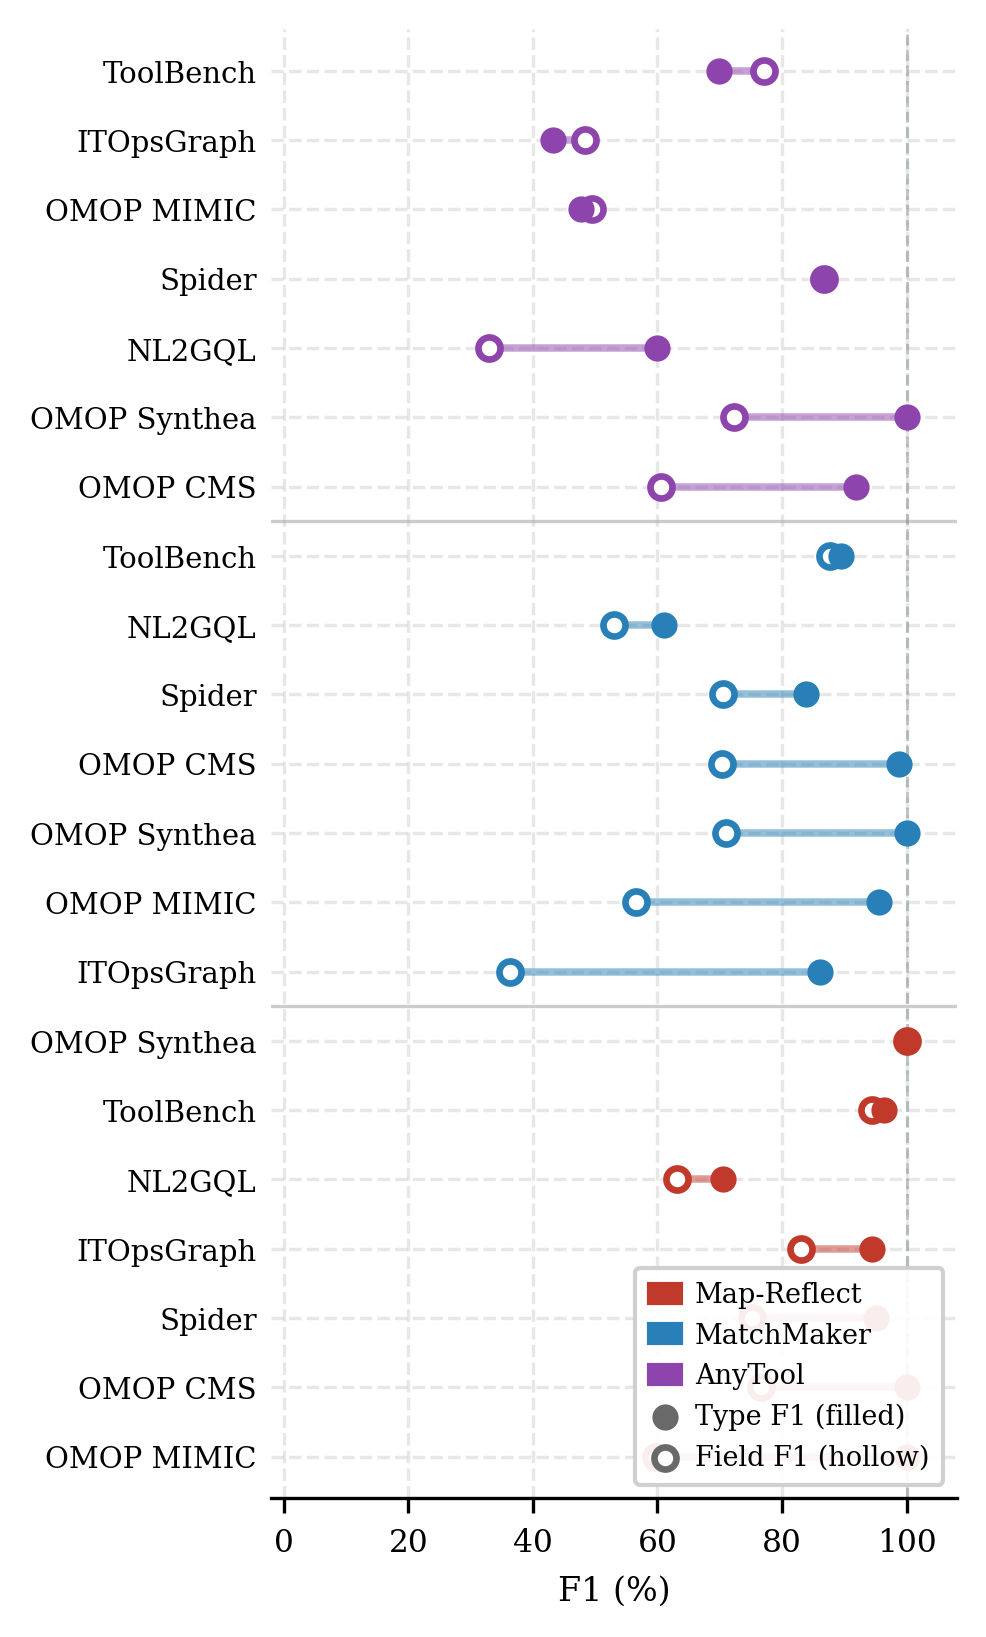
\includegraphics[width=\columnwidth,height=12cm,keepaspectratio]{chart_api_field_gap.png}
    \caption{API-level accuracy (filled) vs.\ field F1 (hollow) across all methods and datasets. Each segment shows the last-mile gap between correctly identifying a schema pair and correctly mapping its fields.}
    \label{fig:api_field_gap}
\end{figure}

\begin{figure}[htbp]
    \centering
    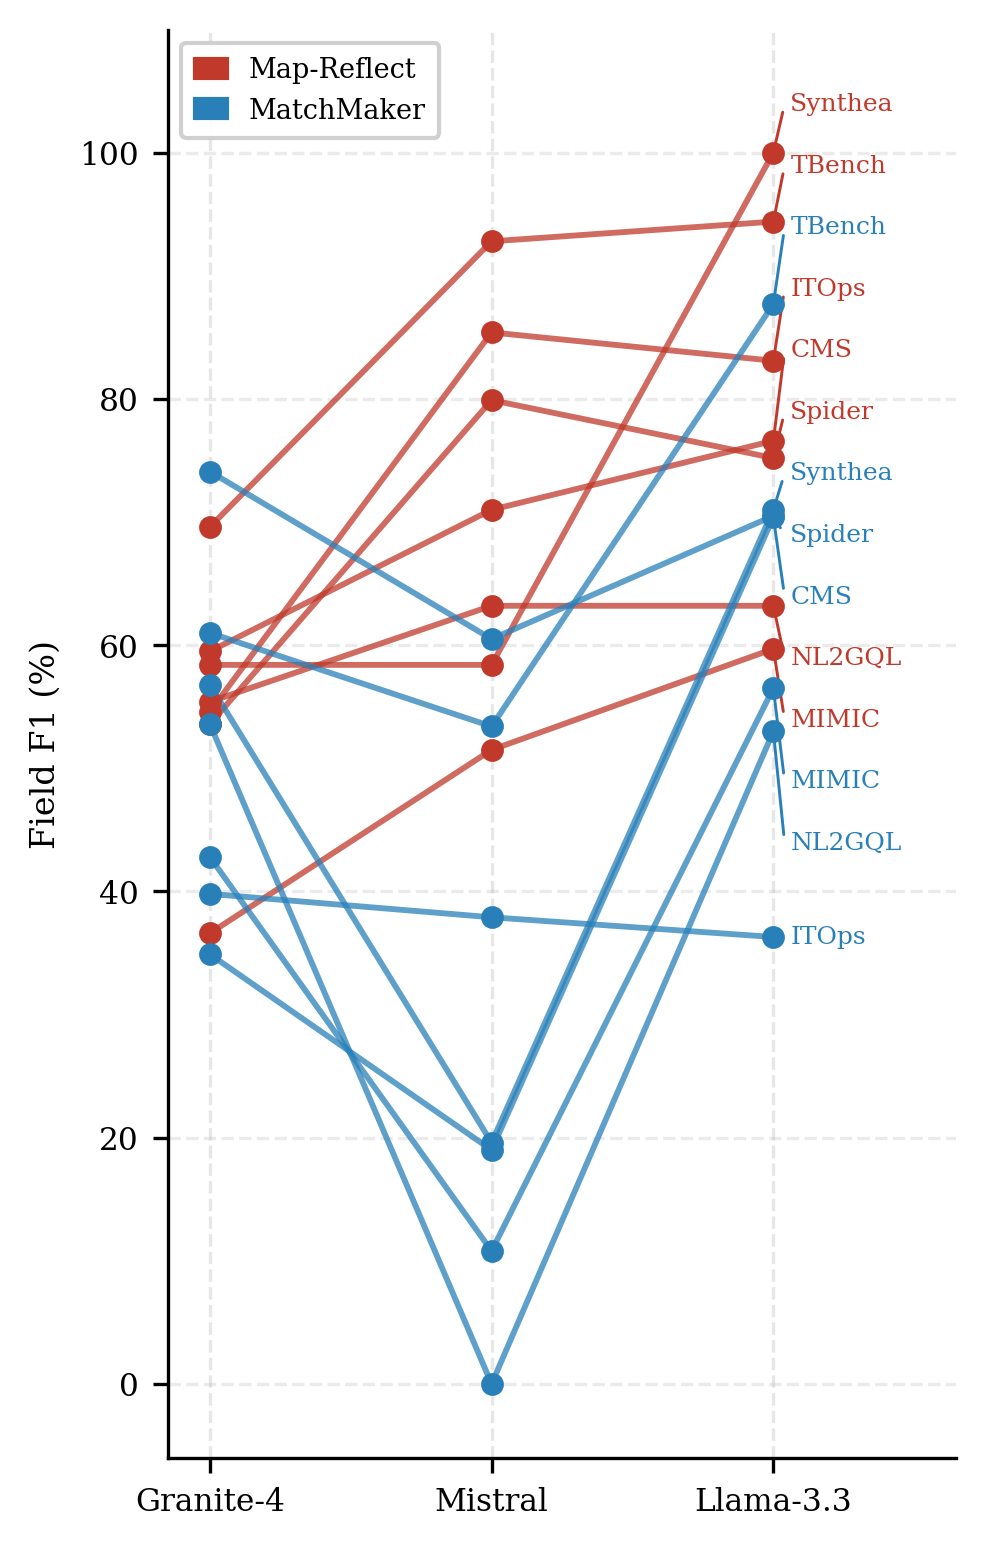
\includegraphics[width=\columnwidth]{chart_method_sensitivity.png}
    \caption{Field F1 by backbone (Granite-4 vs.\ Llama-3.3-70B). MatchMaker NL2GQL Granite selects the correct API on only 57.9\% of samples, illustrating a precision--coverage tradeoff.}
    \label{fig:method_sensitivity}
\end{figure}

\subsection{Ablation Study}\label{sec:ablation}

We conduct ablation studies to isolate the contribution of each reflection signal. Table~\ref{tab:ablation_components} presents the merged ablation across ITOpsGraph, NL2GQL, OMOP-CMS, and OMOP-MIMIC (Llama-3.3-70B). Six representative configurations are shown; four intermediate combinations are omitted as they produce results bracketed by the reported rows.

\textbf{Ablation setup.} The ablation uses a one-prediction-per-field variant: precision is held constant at 86.2\% and field recall varies, directly measuring each signal's net coverage of the many-to-many ground-truth set. The main results tables use the full many-to-many configuration with pruning threshold $\tau_p=0.5$.

\begin{table*}[htbp]
\centering
\small
\caption{Signal ablation (Llama-3.3-70B, field recall \%). Rows ordered by ITOpsGraph recall. Synthea omitted — all nine configurations produce 51.5\% (flat). NL2GQL rows marked \texttt{--} were not evaluated.}
\label{tab:ablation_components}
\begin{tabular}{l ccc rrrr}
\toprule
\textbf{Reflection Trigger} & \textbf{Err} & \textbf{UQ} & \textbf{Nbhd} & \textbf{ITOpsGraph} & \textbf{NL2GQL} & \textbf{CMS} & \textbf{MIMIC} \\
\midrule
Base (no reflection)     & --- & --- & --- & 88.0 & 85.1 & 70.3 & 43.7 \\
UQ-triggered             & --- & \checkmark & --- & \textbf{88.2} & \textbf{85.1} & \textbf{71.0} & 42.9 \\
Self-reflection          & \multicolumn{3}{c}{always} & 82.6 & 83.0 & 71.0 & 42.9 \\
Neighbourhood-triggered  & --- & --- & \checkmark & 80.9 & -- & 70.3 & 42.9 \\
Error-triggered          & \checkmark & --- & --- & 73.1 & -- & 71.0 & \textbf{44.5} \\
Induced (all signals)    & \checkmark & \checkmark & \checkmark & 73.3 & -- & 71.0 & 44.5 \\
\bottomrule
\end{tabular}
\end{table*}

\textbf{Hyperparameter sensitivity.} Varying $\tau_u$ by ${\pm}0.1$ around its value of 0.25 on ITOpsGraph has negligible effect: as Figure~\ref{fig:entropy_dist} shows, the MAP-phase UQ score distribution is heavily right-skewed, with 91.7\% of fields below 0.15 and only 1.0\% above the threshold. The wide gap between the bulk of the distribution and $\tau_u$ means any threshold in the range $[0.15, 0.35]$ produces the same binary gate decisions. The pruning threshold $\tau_p{=}0.5$ is similarly robust: varying it over $\{0.4, 0.5, 0.6\}$ on the ITOpsGraph held-out split changes field F1 by less than 1\,pp. The signal-on/off sweep in Table~\ref{tab:ablation_components} captures the practically meaningful design dimension.

\textbf{Signal contributions.} Reflection is harmful by default and safe only when properly gated. Error-triggered reflection degrades field recall by $-14.9$\,pp: the heuristic patterns (low confidence, ambiguous top-2, type mismatch, etc.) correlate with difficulty but not error, causing the LLM to swap a correct prediction for an alternative. Neighbourhood-triggered reflection degrades by $-7.1$\,pp: on heterogeneous schemas, neighbourhood consistency is not a reliable indicator of error, so the signal fires on correctly-mapped pairs and the LLM over-corrects. Unconditional self-reflection~\cite{shinn2023reflexion} degrades by $-5.4$\,pp for the same reason: prompting the model to critique a correct output produces a rationale for a change that was not needed. Combining error with any other signal compounds the damage; the full three-signal system reaches only 73.3\%. UQ-triggered reflection is the sole safe default: it fires only when candidate uncertainty is genuinely dispersed, targeting cases where reconsidering the top prediction is actually warranted, and never reduces accuracy below the no-reflection baseline.

We compared three gating strategies beyond our heuristic: (i) \textbf{self-consistency}~\cite{wang2023selfconsistency} (majority vote over $k{=}3$ samples at temperature~0.7); (ii) \textbf{SIMBA aggregation-by-classification}~\cite{simba2025} (random forest over pairwise generation similarities); and (iii) \textbf{no gate} (unconditional reflection). Self-consistency achieves $+1.7$\,pp on OMOP-MIMIC from sampling diversity but $-0.9$\,pp on ITOpsGraph — similar to the heuristic but at $3\times$ inference cost. SIMBA identifies near-identical fields as uncertain (61 vs 58 on ITOpsGraph) but produces $-0.2$\,pp — confirming the gate is not the bottleneck; the reflection mechanism lacks new information to exploit. Unconditional reflection degrades by $-5.4$\,pp. Our heuristic gate matches SIMBA coverage at $1\times$ cost, making it the practical recommendation. Because all nine configurations share the same cached MAP predictions, the within-ablation noise floor is below 0.2\,pp; all reported deltas except UQ substantially exceed this floor.

\textbf{OMOP Ablation.} Table~\ref{tab:ablation_components} shows that all signals produce minimal impact on OMOP: deltas range from $-0.8$\,pp to $+0.7$\,pp across all configurations and datasets. Synthea is completely flat — all nine configurations produce identical predictions (51.5\%). OMOP entropy is compressed relative to ITOpsGraph: the model is already near its confidence ceiling on healthcare vocabulary, so the UQ gate fires on 28--45\% of fields but reflection sees the same fixed target schema (OMOP CDM) that MAP already knew — there is no new information available to exploit. The SIMBA experiment confirms this directly: even with a perfectly calibrated uncertainty signal (sampling consistency, not elicited scores), reflection produces $-0.2$\,pp on ITOpsGraph. The bottleneck is the reflection mechanism itself, not the gate. The practical claim for UQ is therefore conservative: it is the only trigger that does not degrade accuracy. On OMOP, where no trigger can help, UQ is neutral; on ITOpsGraph, where there is headroom, it is the only trigger that avoids harm. This is sufficient justification for recommending it as the default.

\begin{figure}[htbp]
    \centering
    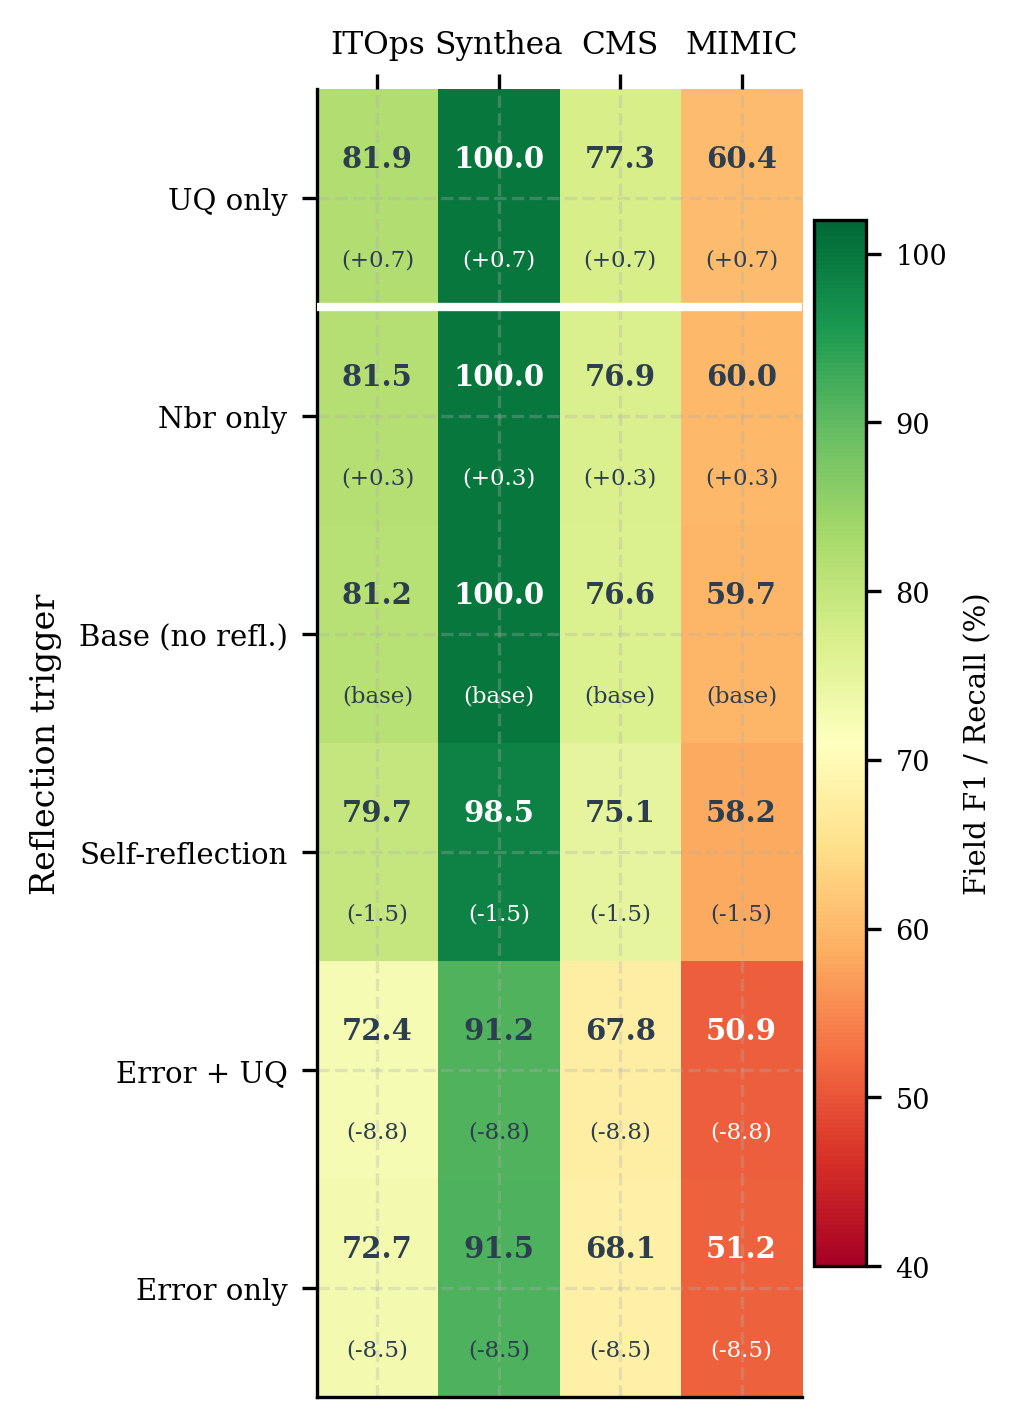
\includegraphics[width=\columnwidth, height=12cm]{chart_signal_heatmap.png}
    \caption{Signal heatmap (Llama-3.3-70B, field recall). White rule separates UQ-only (safe) from configurations that degrade accuracy.}
    \label{fig:signal_heatmap}
\end{figure}

Figure~\ref{fig:signal_heatmap} summarises the full signal ablation. Map-Reflect outperforms MatchMaker on all three OMOP datasets under matched open-source model conditions; the CMS and MIMIC results are the stronger evidence as Synthea has only 12 samples.


\subsection{SchemaNet Per-Pair Analysis}

Tables~\ref{tab:schemanet_type} and~\ref{tab:schemanet} show the per-pair breakdown for SchemaNet, including LLMatch with GPT-4o-mini. Map-Reflect leads on type-level F1 on four of seven pairs. On field-level F1, LLMatch leads on several pairs but uses a materially stronger backbone. AnyTool leads on the non-OMOP pairs (bank1\_bank2, imdb\_sakila) where its hierarchical search is well suited. On the five OMOP-target pairs, all retrieval-based methods degrade because the pairs share the same target pool.

\begin{table}[htbp]
\centering
\small
\setlength{\tabcolsep}{4pt}
\caption{SchemaNet type-level F1, Llama-3.3-70B. $^\ddagger$GNN uses link prediction on the GT graph.}
\label{tab:schemanet_type}
\begin{tabular}{l rrrr}
\toprule
& \textbf{GNN}$^\ddagger$ & \textbf{AnyTool} & \textbf{MM} & \textbf{MR} \\
\midrule
bank1\_bank2      & 29.4 & \textbf{76.5} & 64.7 & 70.6 \\
imdb\_sakila      & 81.2 & 81.2 & 81.2 & \textbf{81.2} \\
cms\_omop         & 17.4 & 47.8 & 15.2 & \textbf{52.2} \\
mimic\_iii\_omop  & 12.1 & 42.0 & 20.1 & \textbf{42.0} \\
synthea\_omop     & 18.4 & 53.1 & 32.7 & \textbf{53.1} \\
cprd\_gold\_omop  & 51.4 & 21.6 & 13.5 & \textbf{23.7} \\
cprd\_aurum\_omop & 15.8 & 21.1 &  2.6 & \textbf{23.7} \\
\midrule
\textbf{Avg}      & 32.2 & \textbf{49.0} & 32.9 & 48.8 \\
\bottomrule
\end{tabular}
\end{table}

\begin{table}[htbp]
\centering
\small
\setlength{\tabcolsep}{4pt}
\caption{SchemaNet field-level F1, Llama-3.3-70B. $^\dagger$LLMatch~\protect\cite{wang2025llmatch} (GPT-4o-mini). $^\ddagger$GNN uses link prediction on GT graph.}
\label{tab:schemanet}
\begin{tabular}{l rrrrr}
\toprule
& \textbf{LLM}$^\dagger$ & \textbf{GNN}$^\ddagger$ & \textbf{AT} & \textbf{MM} & \textbf{MR} \\
\midrule
bank1\_bank2      & 85.0 & 17.6 & \textbf{76.5} & 47.1 & 70.6 \\
imdb\_sakila      & 73.0 & 12.5 & 81.2 & 37.5 & \textbf{81.2} \\
cms\_omop         & 37.0 & 15.2 & 37.0 & 15.2 & \textbf{40.0} \\
mimic\_iii\_omop  & 33.0 &  4.0 & \textbf{29.3} &  7.5 & 26.2 \\
synthea\_omop     & 37.0 &  8.2 & \textbf{30.6} & 16.3 & 25.0 \\
cprd\_gold\_omop  & 30.0 & 10.8 & \textbf{18.9} & 10.8 & 13.5 \\
cprd\_aurum\_omop & 36.0 &  5.3 & 15.8 &  5.3 & \textbf{18.4} \\
\midrule
\textbf{Avg (cond.)} & --- & 10.5 & \textbf{41.3} & 20.0 & 39.3 \\
\bottomrule
\end{tabular}
\end{table}

\subsection{Limitations}

The UQ gate uses a weighted heuristic score $u(f) = 0.3(1-\gamma_1) + 0.3(1-\Delta\gamma) + 0.2\,\mathbb{1}[\text{no reasons}] + 0.06$ over raw LLM-assigned scores, rather than Shannon entropy over a normalised probability distribution or the sampling-based aggregation in SIMBA~\cite{simba2025}. The heuristic fires on the same fields as SIMBA (58 vs 61 on ITOpsGraph), validating that it identifies the same uncertain predictions; but the theoretical linkage to the consistency hypothesis~\cite{xiao2025consistency} is approximate, not exact. WatsonX temperature=0 inference exhibits approximately 5\,pp run-to-run variance on ITOpsGraph (40.9\% of predictions change between independent runs), arising from non-determinism in the serving infrastructure despite temperature=0. Absolute accuracy figures in Tables~\ref{tab:type_results}--\ref{tab:field_results} should therefore be interpreted with a $\pm$5\,pp margin; differences smaller than this should not be treated as significant. Formal confidence intervals were not computed because each dataset has only one ground-truth run (repeating all 521 ITOpsGraph samples three times would triple inference cost); the variance estimate is derived from two independent ITOpsGraph runs. The ablation is not subject to this limitation: the shared-MAP-cache design gives a within-ablation noise floor below 0.2\,pp (only 2--3 of $\sim$965 predictions differ across configurations), making signal comparisons reliable even though absolute numbers carry the 5\,pp margin. Retrieval-mode evaluation uses small target pools (12 products on ITOpsGraph; single fixed target on OMOP), so results there reflect dataset constraints rather than stress-tested discovery. MatchMaker results on ITOpsGraph-MB are limited to a 246-sample subset due to a missing retry mechanism in its agent framework. The conclusion that neighbourhood and error signals are harmful should be understood as specific to the heuristic validators implemented here — a fixed gap threshold of 0.2 and hand-weighted error penalties. Stronger alternatives such as learned graph constraints, cross-validated neighbourhood embeddings, or white-box execution verifiers (where the schema can be deployed and queried) might produce validators that fire more precisely, potentially making these signals safe. We leave this as future work; the current finding establishes a baseline that naive structural signals are unreliable gates, not that structural information is inherently uninformative. Larger retrieval catalogs with hard distractors also remain future work.

\section{Conclusion}

Schema mapping across heterogeneous enterprise APIs and databases is a prerequisite for data federation, tool composition, and agentic workflows, yet it has received less attention than the downstream tasks it enables. Map-Reflect addresses this gap by framing the problem as gated reflection: a greedy Map phase produces an initial alignment, and a Reflect phase refines it selectively using external signals rather than unconditional self-critique. The central finding is that signal quality matters more than reflection itself: error- and neighbourhood-based triggers degrade accuracy by firing on correct predictions, while only uncertainty quantification identifies the cases where reflection genuinely helps. The evaluation spans REST APIs, GraphQL, and relational databases across seven benchmarks including ITOpsGraph and ITOpsGraph-MB, the first human-annotated many-to-many benchmark with bipartite field constraints (786 type pairs, 3,030 fields, 12 products). More broadly, the finding that unconditional self-reflection degrades accuracy generalises to any tool-using agent that revises outputs without external grounding.

\balance
\clearpage
\begin{acks}
We thank John Walczyk, Carlos Eberhardt, Dan Debrunner, Richard Boyer, Phil Renaud, Cesar Araujo, Cheuk Hung Lam, and Sameep Mehta for the discussions and providing the enterprise schemas that have been used in this work.
\end{acks}

\bibliographystyle{ACM-Reference-Format}
\bibliography{sample}

\end{document}
\endinput

